\documentclass[12pt,a4paper]{article}
\usepackage{fontspec}
\usepackage{xeCJK}
\setmainfont{Times New Roman}
\setCJKmainfont{Songti SC}[BoldFont=Heiti SC, AutoFakeBold=2.2]
\setCJKsansfont{Heiti SC}[AutoFakeBold=3.2]
\xeCJKsetup{CJKspace=true}

\usepackage{amsmath,amssymb,bm}
\usepackage{geometry}
\geometry{a4paper,left=2.15cm,right=2.15cm,top=2.05cm,bottom=2.25cm}
\usepackage{setspace}
\setstretch{1.5}
\usepackage{graphicx}
\graphicspath{{extracted_figs/}}
\usepackage{booktabs}
\usepackage{tabularx}
\usepackage{makecell}
\usepackage{array}
\usepackage{caption}
\renewcommand{\figurename}{图}
\renewcommand{\tablename}{表}
\captionsetup{font=small,labelfont=bf,skip=3pt,labelsep=quad}
\usepackage{titlesec}
\usepackage{fancyhdr}
\usepackage{tikz}
\usetikzlibrary{arrows.meta,positioning,calc,fit}
\usepackage{enumitem}
\setlist{nosep,leftmargin=1.7em,itemsep=0.12em,topsep=0.28em}
\usepackage{xcolor}
\usepackage{microtype}
\usepackage{float}

\newcolumntype{L}[1]{>{\raggedright\arraybackslash}p{#1}}
\newcolumntype{Y}{>{\raggedright\arraybackslash}X}

\titleformat{\section}{\sffamily\bfseries\large}{\thesection}{0.55em}{}
\titleformat{\subsection}{\sffamily\bfseries}{\thesubsection}{0.45em}{}
\titleformat{\subsubsection}{\sffamily\bfseries}{\thesubsubsection}{0.4em}{}
\titlespacing*{\section}{0pt}{0.95em}{0.38em}
\titlespacing*{\subsection}{0pt}{0.75em}{0.22em}
\titlespacing*{\subsubsection}{0pt}{0.58em}{0.16em}

\pagestyle{fancy}
\fancyhf{}
\renewcommand{\headrulewidth}{0pt}
\fancyfoot[C]{\thepage}
\fancypagestyle{plain}{\fancyhf{}\renewcommand{\headrulewidth}{0pt}\fancyfoot[C]{\thepage}}

\setlength{\parindent}{2em}
\setlength{\parskip}{0pt}
\setlength{\abovedisplayskip}{5pt}
\setlength{\belowdisplayskip}{5pt}
\setlength{\abovedisplayshortskip}{3pt}
\setlength{\belowdisplayshortskip}{3pt}
\allowdisplaybreaks

\newcommand{\Rmec}{R_{\mathrm{MEC}}}
\newcommand{\Crecv}{C_{\mathrm{recv}}}
\newcommand{\figw}[1]{\includegraphics[width=#1\textwidth]}

\begin{document}

\begin{center}
{\sffamily\bfseries\LARGE 基于交会定位、保证接收域选点与集员在线决策的无线电干扰源自动定位与清除模型}
\end{center}
\vspace{0.55em}

\begin{center}
{\sffamily\bfseries\Large 摘\quad 要}
\end{center}
\vspace{0.25em}
本文针对 2026 年高教社杯全国大学生数学建模竞赛 B 题，围绕“交会定位---检测点选取---在线搜索清除”三个层次建立数学模型，核心结论均经确定性计算或模拟器测试验证。

针对问题一（定位区域直径与覆盖判定），本文把 $\pm 1^{\circ}$ 示向度误差转化为角形区域，用叉积判向等价为两条半平面，把定位区域统一为 $2n$ 条半平面的交（凸集）；显式区分空/有界/无界三态，用旋转卡壳求直径 $D$、Welzl 算法求最小包围圆 $\Rmec$，并证明：存在直径为 $D$ 的圆覆盖定位区域，当且仅当 $\Rmec=D/2$。7 种已知形状验证误差约 $10^{-15}$，2000 组随机交叉验证一致，仿真真实源包含率 100\%。

针对问题二（第二检测点选择），本文由“第一检测点已收到信号 $\Rightarrow$ 接收半径不小于源距”推导保证接收域 $\Crecv$（$d_2\le\max(1000,d_1)$），以最坏定位直径 $J$ 为目标确定性寻优：三构型最优直径 $111.0/41.0/8.2\,\mathrm{m}$，最优第二检测点贴保证接收域外沿以拉大基线、偏角约 $32^{\circ}{\sim}41^{\circ}$；以 $J\le 1.25J_{\min}$ 水平集给出候选区域，两套独立实现互证差不超过 $0.006\,\mathrm{m}$。

针对问题三（全向源在线搜索清除），本文提出“每频道一张可行区域 + 覆盖与清除混排 + 每停重规划”在线策略：\texttt{no\_signal} 只挖本频道、\texttt{direction} 交楔形，三类任务（能清、补测、听洞）按总路程统一调度，停机用“可行域与覆盖任务清空”判定。7 点覆盖网最坏点距 $989\,\mathrm{m}<1000\,\mathrm{m}$，保证每源至少被听见一次。官方三次测试清除 16、13、12 个源，单源耗时 $220.28/258.65/250.17\,\mathrm{s}$。

针对问题四（全向/定向混合源搜索清除），本文针对“无信号不等于无源”，建立位置$\times$朝向联合网格集员表示，构造外环 $1825\,\mathrm{m}$ 包裹 $1800\,\mathrm{m}$ 场地的 N19 超凸包普查站网，配合逆时针顺流、$1300\,\mathrm{m}$ 扇区延迟收割与奔袭静默免听。官方三次测试单源耗时 $575.21/579.18/577.59\,\mathrm{s}$（波幅 $0.69\%$）；本地 1 万局满清率 $99.80\%$、总清除率 $99.98\%$、全向源 $100.00\%$，平均单源 $521.15\,\mathrm{s}/$源。

\vspace{0.35em}
\noindent\textbf{关键词：}交会定位；半平面交；最小包围圆；保证接收域；集员估计；覆盖路径规划；零漏检证书；在线决策

\section{问题重述}
\subsection{问题背景}
无线电干扰源的定位与清除分为初步监测、区域性排查与精准定位三个阶段：前两阶段用固定站、移动监测车或无人机确定干扰源分布区域，最终的精确定位与清除则需技术人员携带便携式测向机在区域内徒步排查。为在危险环境中替代人工，某公司拟研制搭载于机器狗的干扰源自动定位清除系统。

目标区域是以原点为圆心、半径 $1800\,\mathrm{m}$ 的圆形区域（正东为 $x$ 轴、正北为 $y$ 轴，单位米），其中干扰源个数未知，占用互不相同的频道（1--20）；按覆盖角度分为全向源（$360^{\circ}$）与定向源（定向方向两侧各 $90^{\circ}$），有效接收半径在 $1000\sim 1500\,\mathrm{m}$ 之间。测向机测得的示向度为从 $x$ 轴正向逆时针旋转到“检测点指向干扰源”方向的角度，含 $[-1^{\circ},1^{\circ}]$ 误差。机器狗移动速度 $5\,\mathrm{m/s}$、切换频道 $1\,\mathrm{s}$、停测 $5\,\mathrm{s}$、光学定位 $3\,\mathrm{s}$、激光清除 $2\,\mathrm{s}$；距源 $\le 20\,\mathrm{m}$ 方可清除，$\le 5\,\mathrm{m}$ 且位于覆盖角内时无法获得示向度。

\subsection{需要解决的问题}
\begin{enumerate}
\item 问题一：已知若干检测点坐标及某干扰源关于这些检测点的示向度，给出用交会定位法计算多边形定位区域直径（区域内任意两点距离的最大值）的算法，并判断以该直径为直径的圆能否覆盖此区域。
\item 问题二：已知某全向干扰源在一个检测点处的示向度，给出第二个检测点的选择策略与候选区域。
\item 问题三：区域内干扰源均为全向源、总数 10--16 但未知，机器狗从原点出发、初始频道 1，在确保全部清除的前提下使任务时间最短；制定搜索定位清除策略与算法，并经模拟器演练与三次正式测试检验。
\item 问题四：区域内兼有全向与定向干扰源，定向源个数与朝向未知，其余同问题三；给出检测与清除策略及算法并检验。
\end{enumerate}

\section{问题分析}
\subsection{问题一的分析}
交会定位法的本质是方位线交会：每站测得的示向度确定一条方向线，干扰源必在其上；$\pm 1^{\circ}$ 误差使方向线变为张角 $2^{\circ}$ 的角形区域，多站角形区域取交即为定位区域。因此问题一本质是二维半平面交问题，可分解为“区域构造 $\to$ 直径计算 $\to$ 覆盖判定”。关键点有四：(1) 角形区域可精确等价为两条半平面之交，故定位区域必为凸集；(2) 观测可能自相矛盾（区域空）或不足（区域无界），须显式区分空/有界/无界三态；(3) 凸多边形直径必在顶点对取得，可用旋转卡壳 $O(m)$ 求出；(4) 覆盖判定是存在性问题，可用最小包围圆给出严格判据。

\subsection{问题二的分析}
问题二实质是三约束下的最坏情形最小化：一是“听得见”，$S_2$ 须对源可能域内每个可能的源都保证收到信号；二是“交会角不能太小”，两次示向近平行会把区域拉成细长条、直径巨大；三是（可选）留在目标区域内。由 $S_1$ 已收到信号知 $R\ge d_1$，故对远源可放宽到 $1500\,\mathrm{m}$、对近源须保持 $1000\,\mathrm{m}$ 内——“一律按 $1000\,\mathrm{m}$”过保守、“一律按 $1500\,\mathrm{m}$”是假保证；此外定位区域必须裁剪回源可能域与接收上界，否则直径严重虚高；而严格最优只有离散点，故候选区域须用近最优水平集。

\subsection{问题三的分析}
问题三核心是不确定环境下的“搜索---定位---处置”在线决策，可拆为相互耦合的三环节：听见（该频道至少响过一次）、锁住（最小外接圆半径 $\Rmec\le 20\,\mathrm{m}$）、清掉（走进保证盘再激光）。难点有二：一是测向只有角度无距离、多频道否定信息共用可行域易交叉误删，故须每频道独立可行域的集员估计；二是覆盖、定位、清除分布在不同空间位置，须统一调度而非分为先后阶段，故把覆盖义务插入追击路径、每停一次用开路哈密顿路重排下一站；停机不能用剩余源数判定（接口不返回），须用“可行域与覆盖任务清空”规则。

\subsection{问题四的分析}
问题四引入定向源，新增两个难点：一是正负观测信息不对称——正观测（\texttt{direction}）对两类源都给位置楔形约束；负观测（\texttt{no\_signal}）在全向假设下给出“距源超接收半径”的圆盘挖除证书，在定向假设下几乎无位置信息（出扇同样产生 \texttt{no\_signal}）。二是盲区致命——问题三的 7 点网全在圆内，贴边朝外的定向源其可听半平面完全落在圈外。故关键设计为：位置$\times$朝向联合网格集员表示（\texttt{no\_signal} 按朝向衰减、绝不挖盘）、N19 超凸包普查站网（外环 $1825\,\mathrm{m}$ 包裹场地）、逆时针单向顺流 + $1300\,\mathrm{m}$ 扇区延迟收割、奔袭转场静默免听。

\subsection{四个问题之间的联系}
四问构成一条技术链：问题一给出“观测 $\to$ 区域 $\to$ 直径 $\to$ 覆盖判定”的严格几何算法，是全部几何计算的基础模块；问题二给出保证接收域与最坏交会直径的选点方法，为多点序列定位提供粗定位依据（$J_{\min}\approx 111\,\mathrm{m}$ 远大于清除半径 $20\,\mathrm{m}$，故粗定位须交给更精细的在线流程）；问题三、四把几何定位嵌入“搜索---定位---清除”的在线决策闭环，其中问题四叠加定向源的类型推断与零漏检证书。问题三、四的补测点复用问题二的保证接收域，问题四的可行域求交复用问题一的半平面交与最小外接圆算法。

\section{模型假设}
\begin{enumerate}
\item 同平面、源静止：忽略测向机与干扰源的高度差异，二者位于同一平面内；任务期间各源位置、类型、朝向、接收半径、频道均不变。
\item 误差有界：示向度与真实方位角之差落在 $[-1^{\circ},1^{\circ}]$ 内；同一检测点同一频道重复测量的误差保持不变（按站缓存）。
\item 无漏报：源在有效接收半径内且处于覆盖角内时必返回 \texttt{direction} 或 \texttt{near}，故一次 \texttt{no\_signal} 可作为否定证据（问题四中该证据仅对全向假设成立，对定向假设不提供位置信息）。
\item 坐标精确：检测点坐标已知且精确，误差只来源于示向度。
\item 时间可加、转弯可忽略：总时间由移动、停测、切换、清除时间线性叠加。
\item 确定性传播：无遮挡、无随机漏检、无间歇发射，\texttt{no\_signal} 当且仅当“无未清源 / 超出接收半径 / 定向未覆盖”。
\item 保守性（问题三、四）：凡无法连续证明的区域一律保留在可行域内，宁可多测一次也不缩小可行域。
\item 评价口径（问题二）：采用所有相容情形下的最坏值。
\end{enumerate}

\section{符号说明}
\begin{table}[H]
\centering
\begin{tabularx}{\textwidth}{@{}L{4.4cm}Y@{}}
\toprule
\textbf{符号} & \textbf{意义} \\
\midrule
$S_i=(x_i,y_i)$ & 第 $i$ 个检测点坐标（m） \\
$\theta_i/\theta$ & 示向度观测（$^{\circ}$） \\
$G/g$ & 真实干扰源 / 源可能位置 \\
$\Delta/\varepsilon$ & 示向度误差上界（$1^{\circ}$） \\
$W_i=W(S,\theta,\varepsilon)$ & 楔形（角形区域） \\
$P/V/m$ & 定位区域 / 顶点集 / 顶点数 \\
$D$ & 定位区域直径（m） \\
$\Rmec$ & 最小外接圆半径（m） \\
$R$ & 有效接收半径（$1000$--$1500\,\mathrm{m}$） \\
$R_{\mathrm{arena}}$ & 目标区域半径（$1800\,\mathrm{m}$） \\
$\Omega_1$ & 问题二源可能域 \\
$\Crecv$ & 问题二保证接收域 \\
$L(g)$ & 保证接收半径 $\max(1000,\lVert g-S_1\rVert)$（m） \\
$J(q)/J_{\min}$ & 最坏定位直径 / 其最小值（m） \\
$\Omega_k$ & 频道 $k$ 的集员可行域 \\
$B(c,r)$ & 以 $c$ 为心、$r$ 为半径的圆盘 \\
$T$ & 任务总时间（s） \\
$v$ & 移动速度（$5\,\mathrm{m/s}$） \\
$t_{\mathrm{move}},t_{\mathrm{meas}},t_{\mathrm{sw}},t_{\mathrm{clr}}$ & 移动 / 停测 / 切换 / 清除时间（s） \\
$d_{\mathrm{cle}}$ & 光学清除半径（$20\,\mathrm{m}$） \\
$\varphi$ & 定向源朝向（$^{\circ}$） \\
$\mathcal{N}_{19}$ & 问题四 N19 普查站网（19 站） \\
\bottomrule
\end{tabularx}
\end{table}

\noindent 其余符号在首次出现处说明。

\section{数据处理与说明}
本题各问均不涉及外部公开数据集。问题一、二的数据为自建的确定性几何算例与随机仿真（真实源、检测点、示向度误差均按题面规则生成）；问题三的数据来自官方无线电干扰源环境模拟器的演练测试与三次正式测试（案例编码与日志见附录）；问题四的数据来自按官方附件规则逐项一致实现的本地模拟器（与正式接口费率一致，不使用模拟器真值）。本地仿真使用固定随机种子族保证可复现，实验结果与调参/确认集通过种子流与世界签名双重排重，避免数据泄漏。

\section{模型的建立与求解}
\subsection{问题一：交会定位区域直径算法与覆盖判定}
\subsubsection{示向度误差与角形区域模型}
设干扰源真实位置为 $G$，检测点 $S_i=(x_i,y_i)$，从 $S_i$ 指向 $G$ 的真实方位角为
\begin{equation}
\beta(S_i,G)=\operatorname{atan2}(G_y-y_i,\,G_x-x_i)\bmod 360^{\circ}.
\end{equation}
测向机测得示向度 $\theta_i=\beta(S_i,G)+\varepsilon_i$，其中 $|\varepsilon_i|\le\Delta=1^{\circ}$。故真实方位角满足
$\theta_i-\Delta\le\beta(S_i,G)\le\theta_i+\Delta$。
满足此式的一切点构成以 $S_i$ 为顶点、中轴方向为 $\theta_i$、半张角为 $\Delta$ 的角形区域（楔形，图 1）：
\begin{equation}
W_i=\bigl\{P:\beta(S_i,P)\in[\theta_i-\Delta,\,\theta_i+\Delta]\bigr\}.
\end{equation}

\begin{figure}[H]
\centering
\begin{minipage}[t]{0.48\textwidth}
\centering
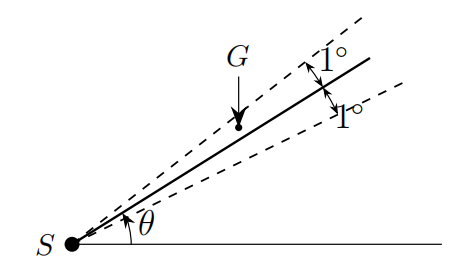
\includegraphics[width=\linewidth]{p07_x59.png}
\caption{干扰源 $G$ 关于检测点 $S$ 的示向度示意图}
\end{minipage}\hfill
\begin{minipage}[t]{0.48\textwidth}
\centering
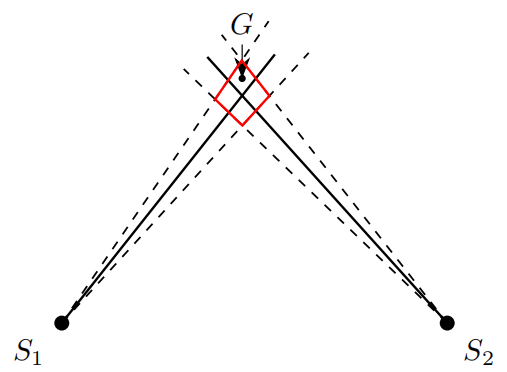
\includegraphics[width=\linewidth]{p07_x60.png}
\caption{交会定位法示意图}
\end{minipage}
\end{figure}

\subsubsection{角形区域到半平面的等价转化}
\textbf{引理 1}（叉积判向）\quad 设 $\mathbf{u}(\alpha)=(\cos\alpha,\sin\alpha)$，则 $P$ 相对 $S_i$ 的方位角 $\ge\alpha$（位于方向 $\alpha$ 的逆时针一侧）当且仅当
\begin{equation}
\operatorname{cross}\bigl(\mathbf{u}(\alpha),\,P-S_i\bigr)=\cos\alpha(P_y-y_i)-\sin\alpha(P_x-x_i)\ge 0.
\end{equation}
由引理 1，角形区域可精确等价（非近似）为两条半平面之交 $W_i=H_i^{(1)}\cap H_i^{(2)}$：令 $\alpha_i=\theta_i-\Delta$、$\gamma_i=\theta_i+\Delta$，两半平面的内法向量分别为 $(-\sin\alpha_i,\cos\alpha_i)$ 与 $(\sin\gamma_i,-\cos\gamma_i)$，均以 $ax+by+c\ge 0$ 为可行方向。于是 $n$ 个检测点给出 $2n$ 条半平面，定位区域为
\begin{equation}
P=\bigcap_{i=1}^{n}W_i=\bigl\{P:a_jx+b_jy+c_j\ge 0,\; j=1,2,\ldots,2n\bigr\}.
\end{equation}
两个检测点 $S_1,S_2$ 交会定位的几何示意如图 2 所示。

\textbf{性质 1}（凸性）\quad 有限个半平面的交必为凸集；非空时为（可能有界、无界的）凸多边形。

\subsubsection{半平面交与状态判定}
算法采用边界线交点枚举 + 凸包 + 衰退锥判定，对“空 / 有界 / 无界”三态均给出正确结果，且不引入人为截断：
\begin{enumerate}
\item 顶点枚举：对每对边界直线 $\ell_j,\ell_k$，若 $\det_{jk}=a_jb_k-a_kb_j\neq 0$ 则求交点，筛选满足全部约束（容差 $\varepsilon=10^{-9}$）的候选顶点集 $Q$；有界非退化时 $P=\operatorname{conv}(Q)$。
\item 有界性判定（衰退锥判据）：定义衰退锥 $\mathcal{C}=\{\mathbf{d}:\mathbf{n}_j\cdot\mathbf{d}\ge 0\}$（$\mathbf{n}_j$ 为内法向量），$P$ 有界当且仅当 $\mathcal{C}=\{0\}$；将内法向量幅角升序排列，记最大循环间隔 $G_{\max}$，则 $P$ 有界 $\Leftrightarrow G_{\max}<180^{\circ}$。该判据避免了“用固定方框截断真实区域”的错误。
\end{enumerate}

\subsubsection{直径计算（旋转卡壳）}
凸多边形直径定义为 $D=\max_{p<q}\lVert v_p-v_q\rVert_2$。\textbf{引理 3}：凸紧集上距离最远的两点可分别取为顶点，故只需枚举顶点对。利用“对踵点对”的单调性，旋转卡壳算法在 $O(m)$ 时间内求出直径。

\subsubsection{最小包围圆（Welzl 随机增量算法）}
最小包围圆 $(\mathbf{c}^{*},\Rmec)=\arg\min_{\mathbf{c}}\max_{v}\lVert v-\mathbf{c}\rVert_2$ 由 $V$ 中 2 或 3 个点唯一确定（两点为直径、三点为外接圆）。Welzl 算法随机打乱顶点、增量维护支撑集 $B$（$|B|\le 3$），期望时间 $O(m)$。

\subsubsection{覆盖判定：核心定理}
\textbf{定理 4}（覆盖判定定理）\quad 存在直径为 $D$ 的圆覆盖定位区域 $P$，当且仅当 $\Rmec=D/2$。

证明：充分性——取最小包围圆圆心 $\mathbf{c}^{*}$、半径 $D/2$ 即得覆盖圆；必要性——若存在半径 $D/2$ 的圆覆盖 $P$，则 $\Rmec\le D/2$；又因 $P$ 含一对相距 $D$ 的直径端点，任何覆盖 $P$ 的圆半径必 $\ge D/2$，故 $\Rmec\ge D/2$。两式合并即得 $\Rmec=D/2$（数值容差内）。

\subsubsection{算例求解结果}
取七种典型构型（东西/南北对望、直角、同侧、$120^{\circ}$ 环绕、共线环绕、东/北/西），示向度取指向原点方向、误差 $\pm 1^{\circ}$。结果：正对交会区域为细长菱形，$\Rmec=D/2$，能覆盖；直角交会区域极小（$D\approx 49.39\,\mathrm{m}$）且能覆盖，可见交会角接近 $90^{\circ}$ 时定位最精确；多站环绕区域为六边形，$\Rmec>D/2$，不能覆盖；同侧构型交集无界，算法正确返回“无界”。

\begin{figure}[H]
\centering
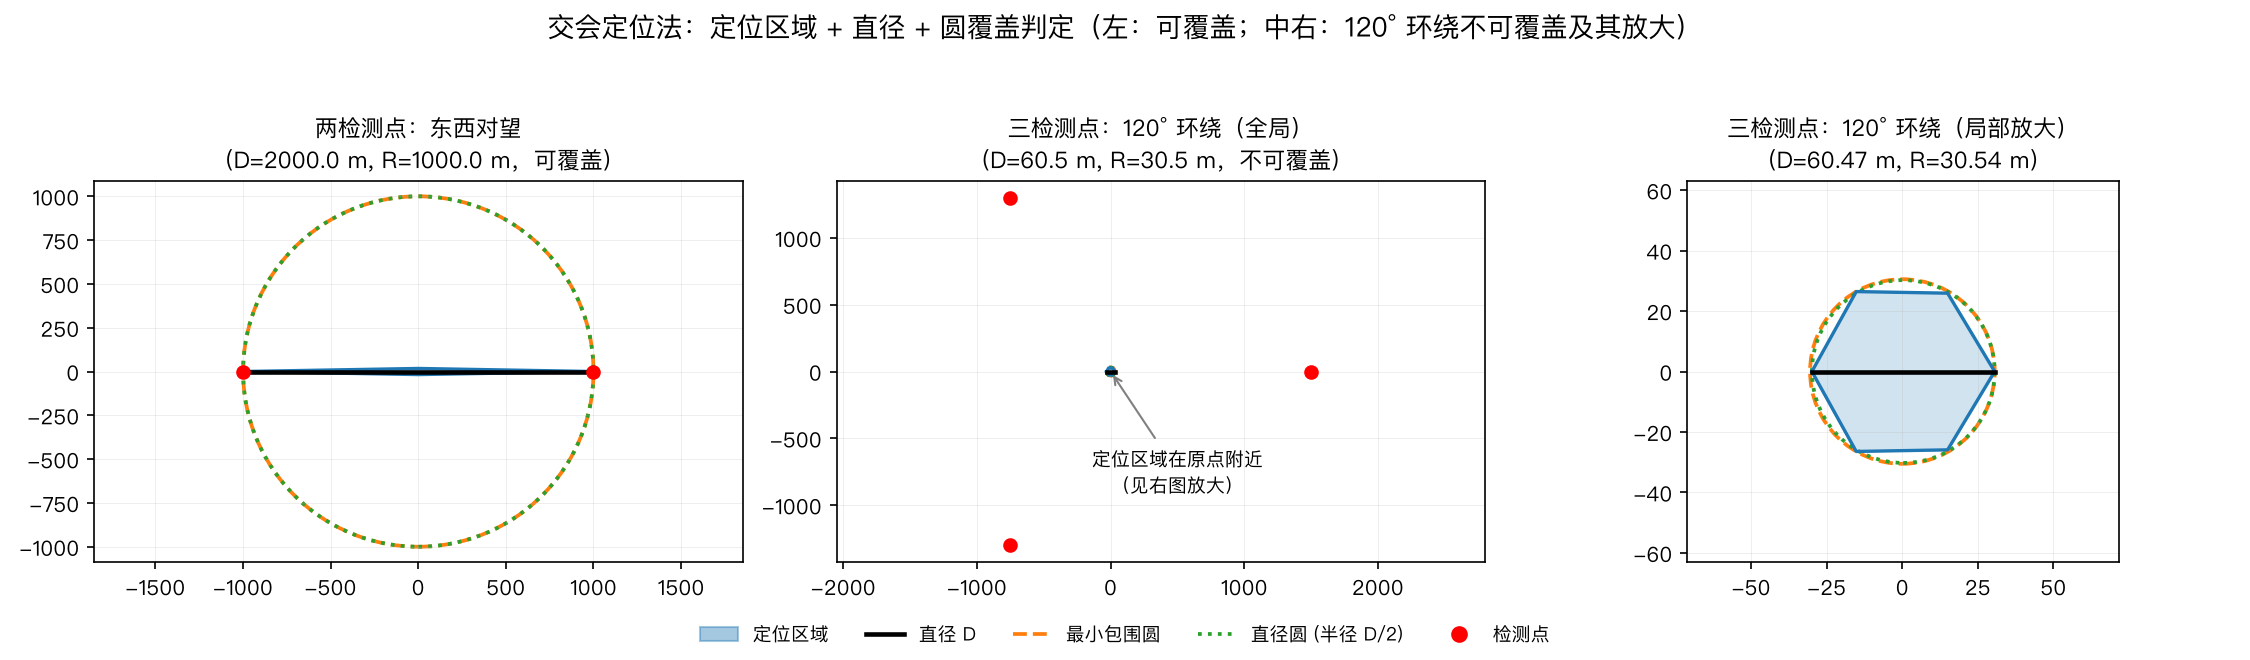
\includegraphics[width=0.96\textwidth]{p09_x76.png}
\caption{交会定位算例：定位区域、直径、最小包围圆与直径圆}
\end{figure}

\subsection{问题二：第二检测点选择策略与候选区域}
\subsubsection{源可能域 $\Omega_1$}
第一次观测给出示向度，源必位于沿示向线、张角 $2^{\circ}$ 的楔形内；$S_1$ 收到信号要求 $5<d_1\le R\le 1500$；源又在目标圆内。故
\begin{equation}
\Omega_1=\bigl\{g:\lVert g\rVert\le 1800,\; 5<\lVert g-S_1\rVert\le 1500,\; \lvert\operatorname{wrap}(\angle(g-S_1)-\theta_1)\rvert\le 1^{\circ}\bigr\}.
\end{equation}
注意目标圆以原点为心、不以 $S_1$ 为心，楔形内各方向被目标圆截断的距离不同，须逐方向计算远端距离 $r_{\mathrm{far}}(\phi)=\min(1500,\,\text{该方向穿出目标圆的距离})$。

\subsubsection{保证接收域 $\Crecv$}
$S_2$ 的“听得见”必须对 $\Omega_1$ 内每个可能的源都成立。由 $S_1$ 已收到信号知 $R\ge d_1$ 且 $R\le 1500$，要使 $S_2$ 对一切相容的 $R$ 都能收到 $g$，必须且只需 $d_2\le\max(1000,d_1)$。由此定义
\begin{equation}
\Crecv=\Bigl\{q:F(q)=\sup_{g\in\Omega_1}\bigl(\lVert q-g\rVert-L(g)\bigr)\le 0\Bigr\},\qquad
L(g)=\max\bigl(1000,\lVert g-S_1\rVert\bigr).
\end{equation}
几何上 $\Crecv$ 近似“三圆叶子” $B(S_1,1000)\cap B(P_{-},1000)\cap B(P_{+},1000)$（$P_{\pm}$ 为 $\pm 1^{\circ}$ 方向上 $1000\,\mathrm{m}$ 远弧两端），该三圆交是 $\Crecv$ 的保守充分条件。

\subsubsection{最坏定位区域直径 $J$（含后验裁剪）}
第二次观测后定位区域为
\begin{equation}
\Omega_2=W_1\cap W_2\cap\Omega_1\cap\{5<\lVert z-q\rVert\le 1500\},
\end{equation}
其中裁剪回 $\Omega_1$ 排除了 $d_1>1500\,\mathrm{m}$ 的不可能位置、裁剪 $d_2\le 1500$ 排除了 $S_2$ 收不到的位置。目标取所有可能源、所有相容第二次误差下的最坏值：
\begin{equation}
J(q)=\sup_{g\in\Omega_1}\sup_{e_2\in[-1^{\circ},1^{\circ}]}\operatorname{diam}\bigl(\Omega_2(q,g,e_2)\bigr).
\end{equation}
后验裁剪的必要性：若不裁剪，中心构型 $S_2=(800,600)$ 处最坏情形的后验四顶点中有三个离 $S_1$ 达 $1551$--$1623\,\mathrm{m}$（物理不可能），未裁剪直径被虚高至 $134.98\,\mathrm{m}$；裁剪后退化为真源附近的单点，最坏直径降至 $112.1\,\mathrm{m}$。

\subsubsection{求解与结果}
$J$ 取有限源网格 $\times$ 有限误差网格上的最大值（确定性网格离散，逐位可复现），在保证接收域内做 $25\,\mathrm{m}\to 5\,\mathrm{m}\to 1\,\mathrm{m}\to 0.5\,\mathrm{m}$ 多级细化寻优。三构型结果如下：

\begin{table}[H]
\centering
\caption{问题二三构型求解结果}
\small
\begin{tabularx}{\textwidth}{@{}L{3.15cm}L{1.35cm}L{3.15cm}L{2.55cm}Y@{}}
\toprule
\textbf{构型} & $\boldsymbol{J_{\min}}$\textbf{/m} & \textbf{最优} $\boldsymbol{S_2}$ & \textbf{离} $\boldsymbol{S_1}$\textbf{/偏角} & \textbf{1.25 候选区} \\
\midrule
中心 $(0,0)$，$0^{\circ}$
  & 111.0 & $(844,\pm 544)$ & $1004\,\mathrm{m}/32.8^{\circ}$
  & $855$--$1004\,\mathrm{m}$ / $16.1^{\circ}$--$60.1^{\circ}$ \\[0.35em]
向外 $800$ $(-1000,0)$，$180^{\circ}$
  & 41.0 & $(-1594.8,\pm 511.4)$ & $784\,\mathrm{m}/40.7^{\circ}$
  & $593$--$1000\,\mathrm{m}$ / $24.4^{\circ}$--$60.8^{\circ}$ \\[0.35em]
切向 $(1790,0)$，$90^{\circ}$
  & 8.2 & $(1688.4,+120.5)$ & $158\,\mathrm{m}/40.1^{\circ}$
  & $125$--$236\,\mathrm{m}$ / $31.0^{\circ}$--$60.3^{\circ}$（西侧一瓣） \\
\bottomrule
\end{tabularx}
\end{table}

三个构型的几何含义一致：最优 $S_2$ 均“贴保证接收域外沿、偏角 $32.8^{\circ}{\sim}40.7^{\circ}$”，在基线长度与交会角之间取得折中。最坏情形见证（三构型一致）：最坏直径出现在楔形远弧端点（$\phi=\pm 1^{\circ}$、$d_1=r_{\mathrm{far}}$）$\times$ 第二次误差极值（$e_2=\pm 1^{\circ}$）处。

\begin{figure}[H]
\centering
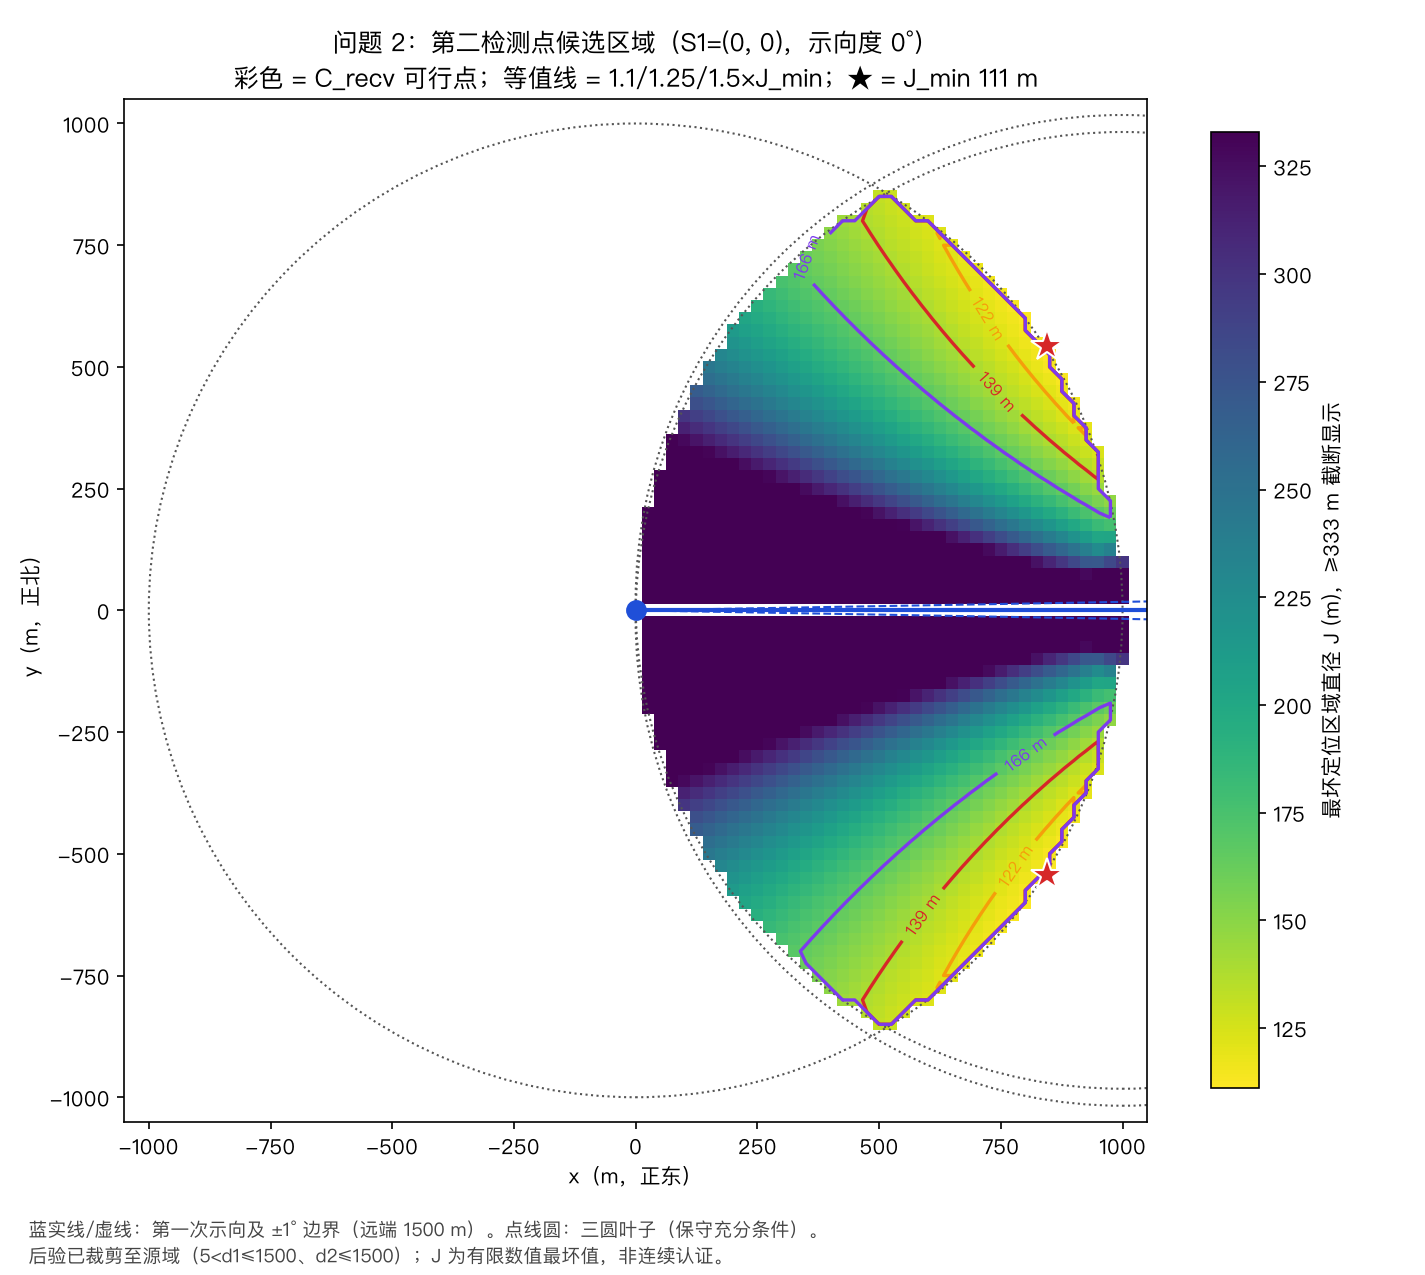
\includegraphics[width=0.78\textwidth]{p12_x99.png}
\caption{中心构型候选区域（彩色为可行域最坏直径，等值线为 $1.1/1.25/1.5\times J_{\min}$，$\star$ 为最优点）}
\end{figure}

\begin{figure}[H]
\centering
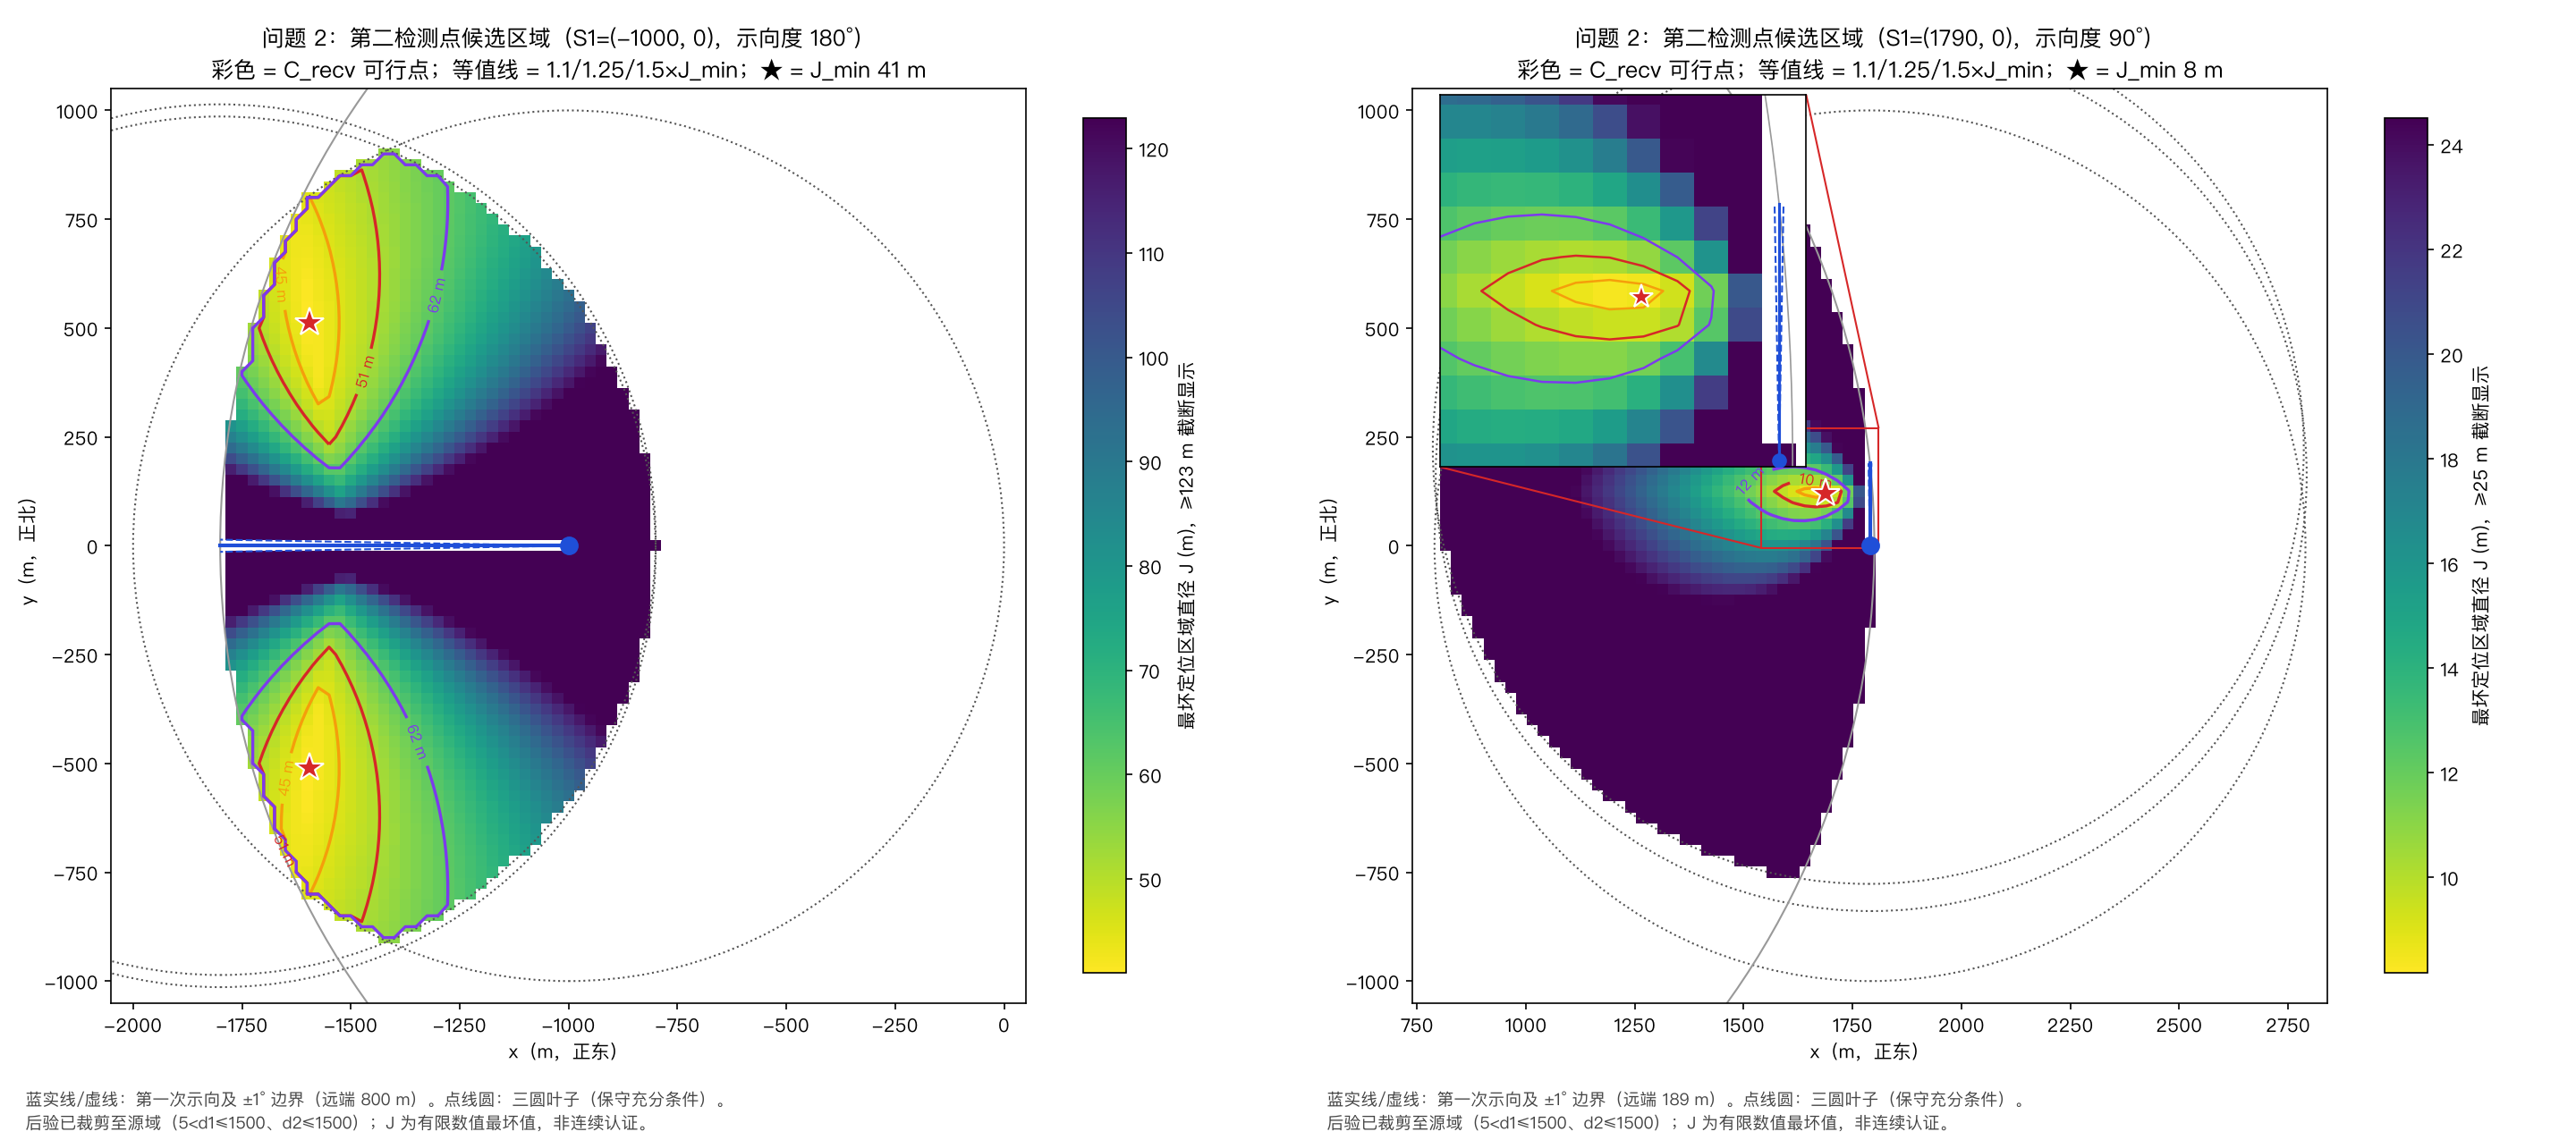
\includegraphics[width=0.96\textwidth]{p12_x100.png}
\caption{向外 $800\,\mathrm{m}$（左）与切向边界（右）构型候选区域}
\end{figure}

\subsubsection{候选区域：近最优水平集}
严格最优只有离散的点，单点交不了“候选区域”这道题，故把“较好”放宽为近最优水平集
\begin{equation}
\mathcal{R}_{\alpha}=\bigl\{S_2\in\Crecv:J(S_2)\le\alpha J_{\min}\bigr\}.
\end{equation}
$\alpha=1.25$ 允许最坏直径比最优差 $25\%$（中心构型 $111\to 139\,\mathrm{m}$），属建模容差而非题面常数。敏感性分析表明 $\alpha\in[1.1,1.5]$ 时候选区域始终是贴外沿的两瓣，只改变向内伸入深度，策略结论不依赖 $\alpha$ 的精确取值。

\subsection{问题三：全向干扰源在线搜索清除策略}
\subsubsection{覆盖网：最坏 $1000\,\mathrm{m}$ 的等圆覆盖}
单次任务总时间 $T=t_{\mathrm{move}}+t_{\mathrm{meas}}+t_{\mathrm{sw}}+t_{\mathrm{clr}}$，其中 $t_{\mathrm{move}}=L/v$。移动时间约占总时间的 $77\%$，故缩短总时间的关键是缩短移动路程。为保证场地上任意位置的源都至少被听见一次，覆盖点须满足“场地内任意点到最近覆盖点的距离 $\le 1000\,\mathrm{m}$”，即等圆覆盖圆盘问题。对 $n=6$ 个等圆，最小覆盖半径 $0.5559\times 1800\approx 1000.6\,\mathrm{m}$ 略超 $1000\,\mathrm{m}$，盖不住；对 $n=7$，最小覆盖半径 $900\,\mathrm{m}<1000\,\mathrm{m}$，盖得住。故 7 点覆盖网是最小完备配置。最终取原点 + 半径 $1150\,\mathrm{m}$ 正六边形共 7 点（把外圈半径外扩到 $1150\,\mathrm{m}$ 使覆盖点更贴近均匀分布的外圈源、减少追击往返），此时最坏覆盖距离
\begin{equation}
d_{\max}=\sqrt{1150^{2}+1800^{2}-2\cdot 1150\cdot 1800\cos 30^{\circ}}\approx 989\,\mathrm{m}<1000\,\mathrm{m}.
\end{equation}
7 点网保证最坏 $R=1000\,\mathrm{m}$ 时每只源至少被听见一次；注意这只保证“听见”、不保证“清除”。否定证据取 $990\,\mathrm{m}$（而非 $1000\,\mathrm{m}$），为 $10\,\mathrm{m}$ 格点半对角误差留出工程余量，保证 \texttt{no\_signal} 挖洞必不误删真实源。

\begin{figure}[H]
\centering
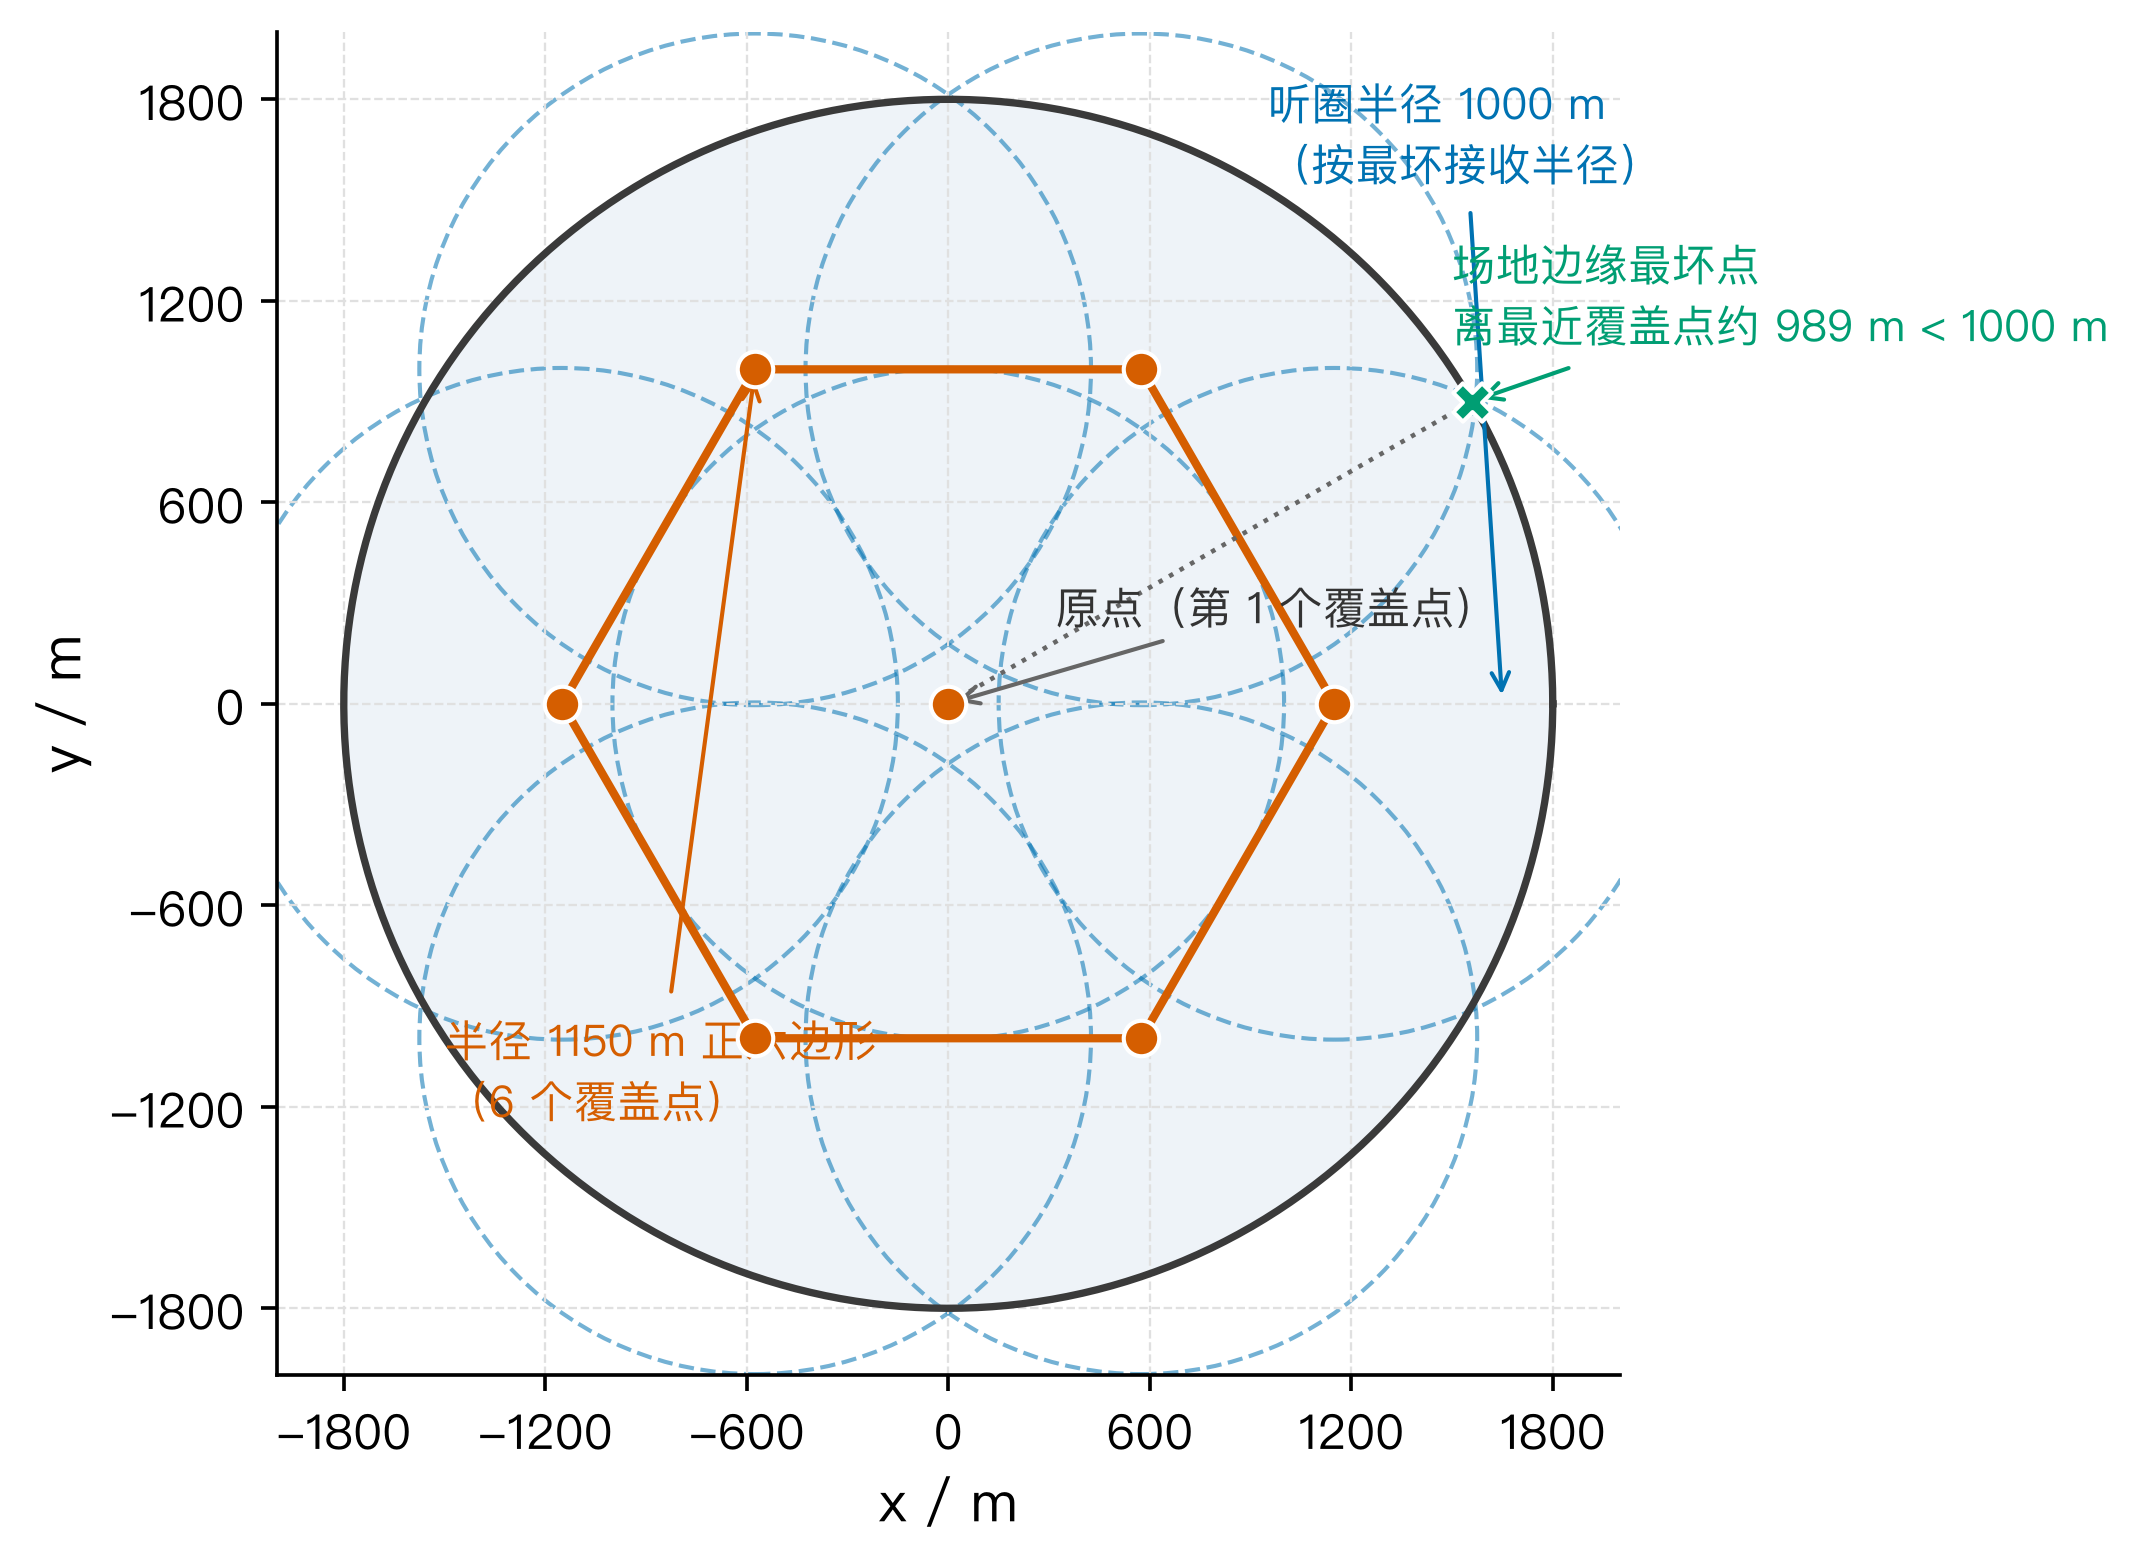
\includegraphics[width=0.72\textwidth]{p14_x110.png}
\caption{七点覆盖网（原点 + 半径 $1150\,\mathrm{m}$ 正六边形，听圈半径 $1000\,\mathrm{m}$）}
\end{figure}

\subsubsection{每频道一张可行区域（集员估计）}
对频道 $k$ 维护一张可行区域 $\Omega_k$（集合而非概率分布），初始 $\Omega_k^{(0)}=B(O,R_{\mathrm{arena}})$。每得到一次测量按以下规则收缩：
\begin{itemize}
\item \texttt{no\_signal}：源距 $S$ 超过其接收半径（$\ge 1000\,\mathrm{m}$，工程取 $990\,\mathrm{m}$），只从本频道挖掉 $B(S,990)$；
\item \texttt{direction}（示向度 $\theta$）：源落在 $\theta\pm 1^{\circ}$ 楔形内且距 $S$ 不超过 $1500\,\mathrm{m}$，
$\Omega_k\leftarrow\Omega_k\cap W(S,\theta,1^{\circ})\cap B(S,1500)$；
\item \texttt{near} 或清除成功：该频道结案。
\end{itemize}
楔形为两条边界射线的两个半平面之交：
\begin{equation}
W(S,\theta,\varepsilon)=\bigl\{P:\mathbf{u}(\theta-\varepsilon)\times(P-S)\ge 0,\;
\mathbf{u}(\theta+\varepsilon)\times(P-S)\le 0\bigr\}.
\end{equation}
关键一点：\texttt{no\_signal} 挖洞只挖本频道自己的可行域，不能把别的未听频道一并挖掉，否则一个频道的否定信息会误删另一个尚未被听见的源。每个频道最多保留 4 条示向度参与求交（按角度多样性择优选留）。当可行域顶点集的最小外接圆半径 $\Rmec\le 20\,\mathrm{m}$ 时，源已“锁住”，从圆心 $c$ 进入保证盘 $B(c,20-\Rmec)$ 内执行清除。

\subsubsection{三类任务混排与每停一次重规划}
每一停，机器狗从当前点对手头任务求一条开路最短哈密顿路（不回起点），只走其中的下一站，到达后重新规划。三类任务为：
\begin{enumerate}
\item 能清 $\mathcal{T}_{\mathrm{clear}}$：$\Rmec\le 20$，目标进入保证盘；
\item 补测/探点 $\mathcal{T}_{\mathrm{station}}$：只有一条楔形或定位区域仍太大，补测站概念上是问题二的保证接收域 $\Crecv$，实现上取沿示向离开约 $1000\,\mathrm{m}$、偏开 $\pm 30^{\circ}$ 的候选点；
\item 听洞 $\mathcal{T}_{\mathrm{cover}}$：贪心集合覆盖后仍需要去的普查点。
\end{enumerate}
开路最短哈密顿路在任务点数 $\le 16$ 时用 Held--Karp 算法精确求解（状态转移
\begin{equation}
dp[\mathrm{mask}][j]=\min_{i\in\mathrm{mask},\,i\neq j}\bigl(dp[\mathrm{mask}\setminus\{j\}][i]+d_{ij}\bigr),
\end{equation}
点数更多时用 2-opt 启发式。对已能清除的源，其“城市”是保证盘而非单点，进入点取盘边界上离上一站最近的点。同一站能测的测完、能清的清完再走，没有固定优先级。

\subsubsection{停机规则}
官方接口不返回“还剩几只”，任务结束不能按剩余个数判定。本文停机规则：所有已听见的频道要么已清除、要么不再追击，且 7 点覆盖网上不存在仍需听的洞；或已听见 16 只源（题面上限）。这是充分停机条件（“按本文规则已无待办任务”），而非“场上已无源”的完备证明。

\subsubsection{求解结果}
\begin{table}[H]
\centering
\caption{问题三本地 10000 局方法对比（非官方模拟器）}
\small
\begin{tabularx}{\textwidth}{@{}Yccccc@{}}
\toprule
\textbf{策略} & \textbf{清完率} & \textbf{均时/s} & \textbf{中位/s} & \textbf{均走/m} & \textbf{平均检测/次} \\
\midrule
静态对照：先 7 点普查再清 & 99.72\% & 5512 & 5410 & 22536 & 155.2 \\
早期动态（未加固） & 98.74\% & 4340 & 4287 & 16617 & 158.7 \\
上场：可行域 + 混排（停机规则） & 99.95\% & 3431.9 & 3407.3 & 13252 & 119.7 \\
\bottomrule
\end{tabularx}
\end{table}

本策略较静态对照平均缩短 $5512-3431.9=2080\,\mathrm{s}$（约 $38\%$），且清完率更高；早期动态虽更快但清完率降至 $98.74\%$，说明仅追求走路最短、不加可行域加固会引入漏清。

\begin{figure}[H]
\centering
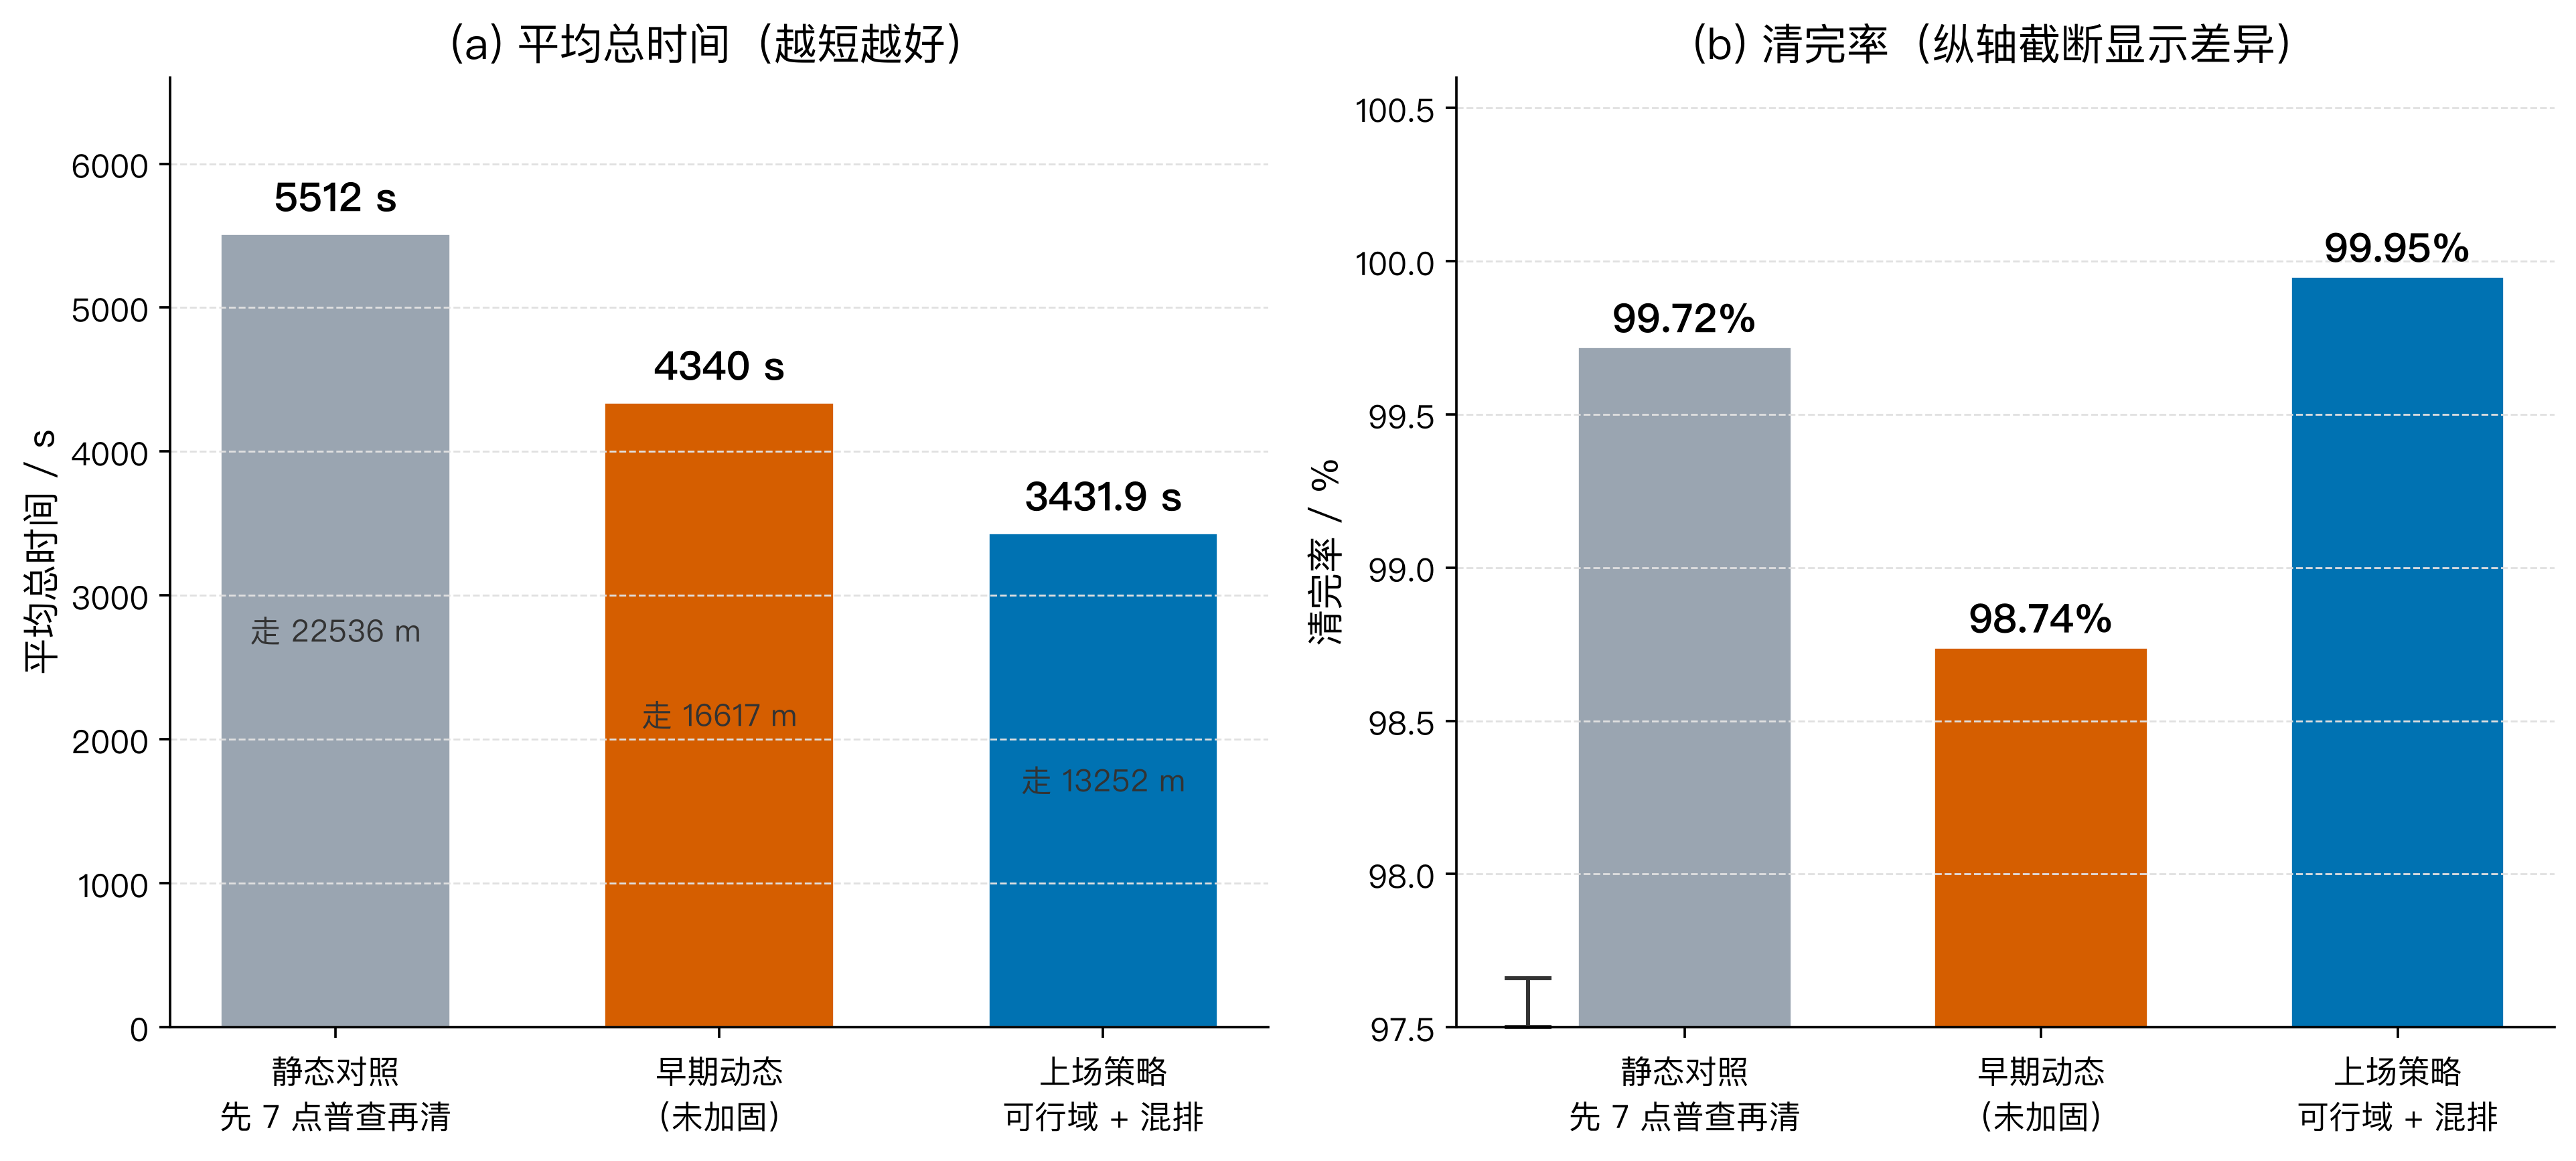
\includegraphics[width=0.96\textwidth]{p16_x121.png}
\caption{三种策略的清完率与平均总时间对比（本地 10000 局，非官方；按停机规则停机）}
\end{figure}

\begin{figure}[H]
\centering
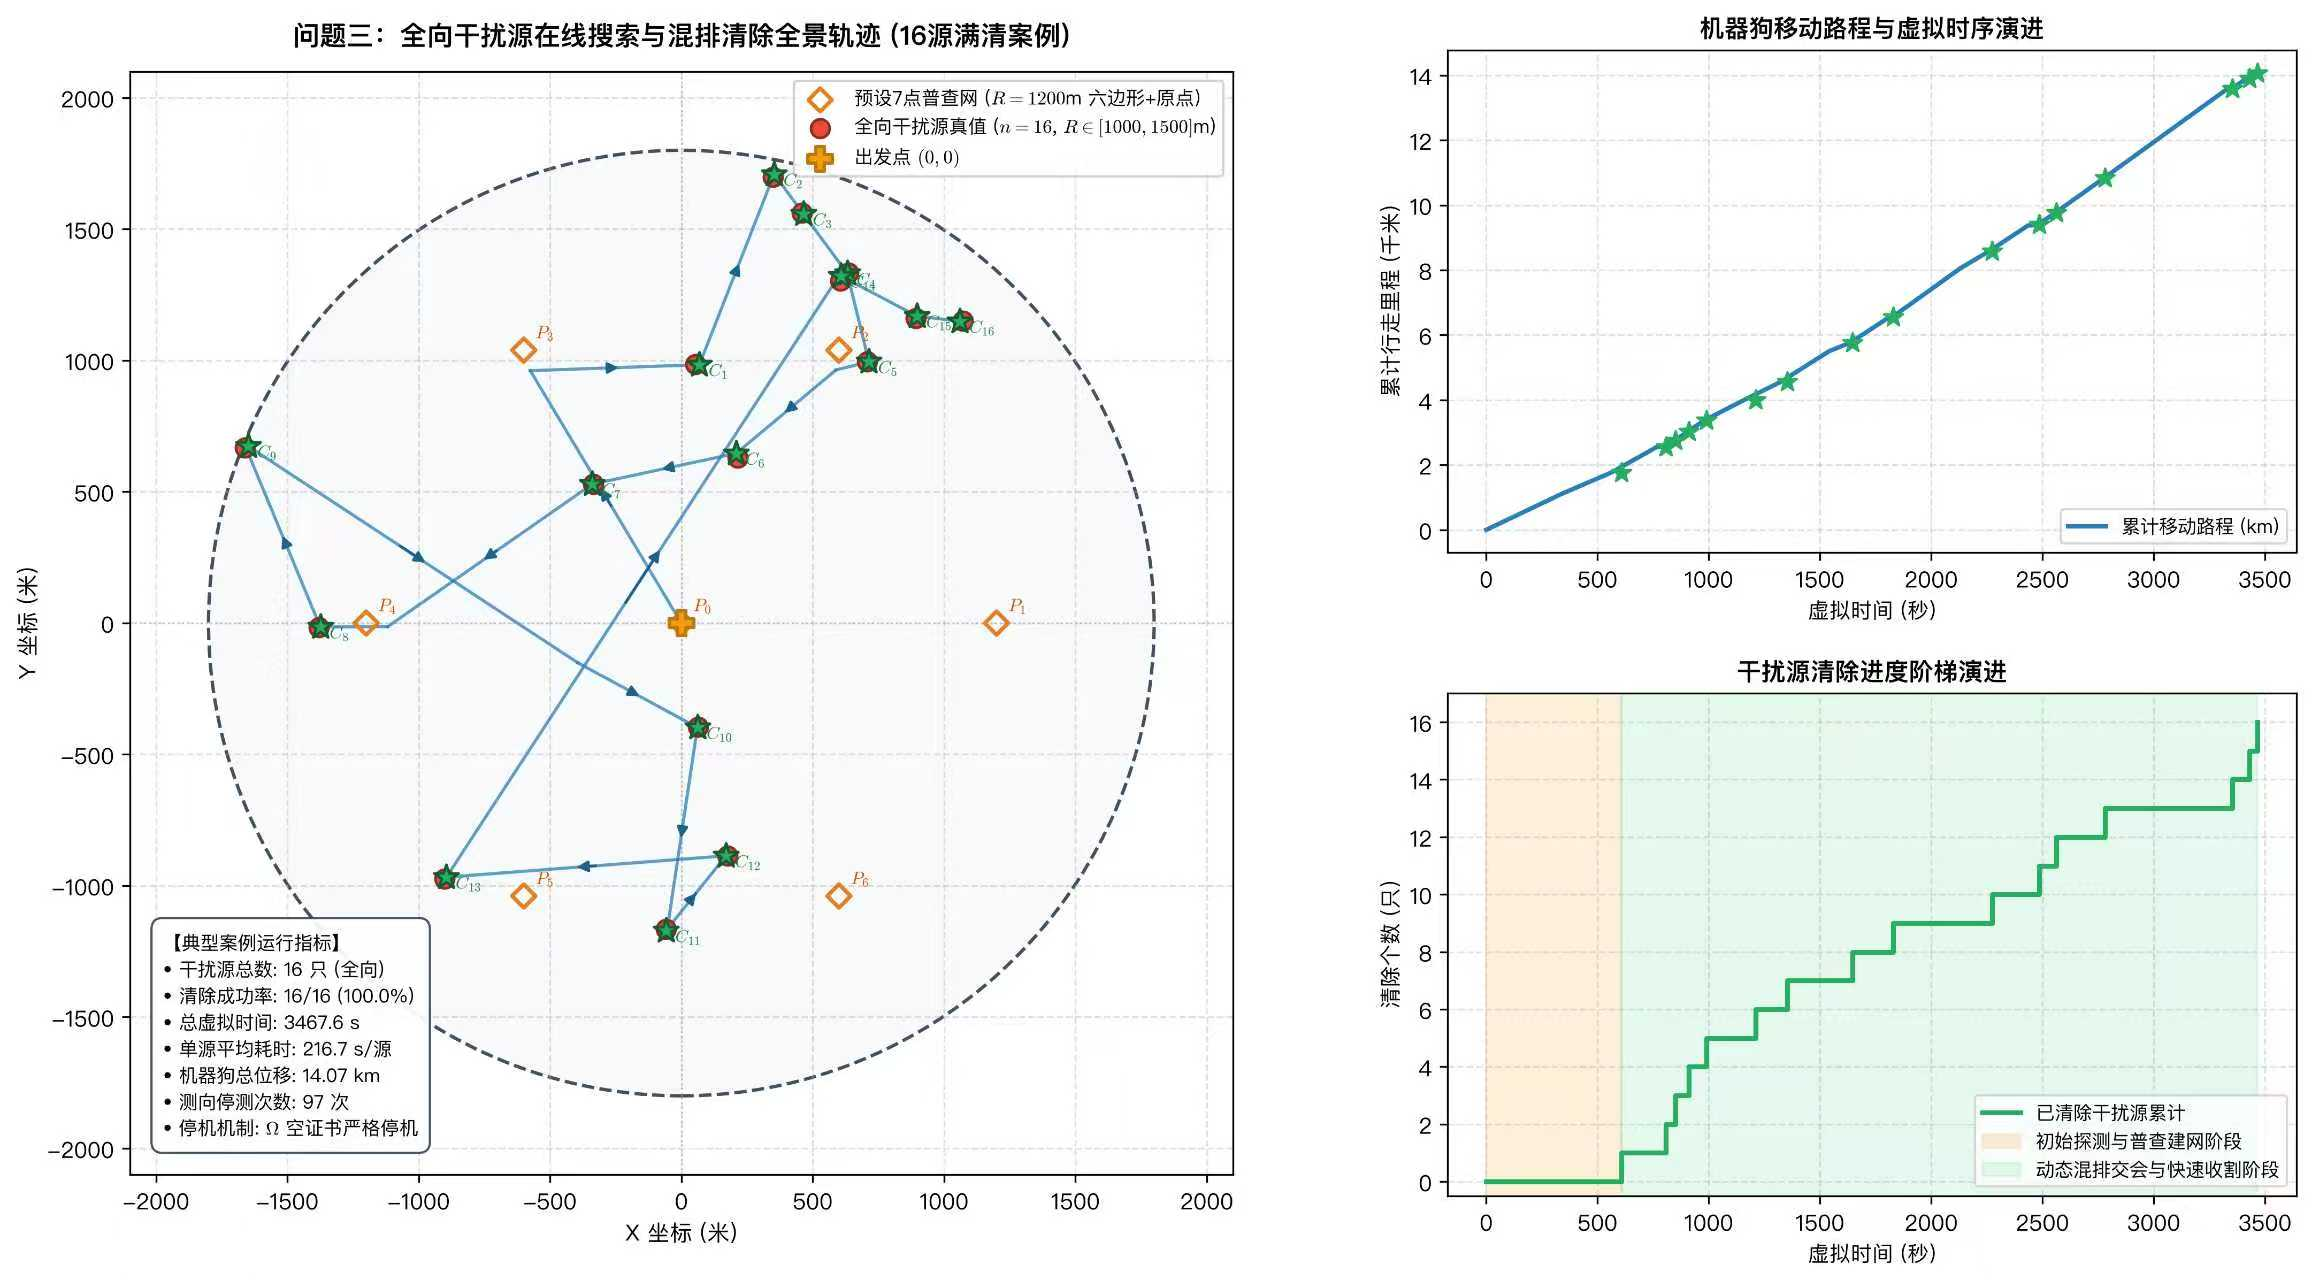
\includegraphics[width=0.92\textwidth]{p17_x126.jpeg}
\caption{问题三全向干扰源在线搜索与混排清除全景轨迹与时序演进图}
\end{figure}

图 8 给出 16 个全向干扰源极端规模场景下的典型仿真轨迹（种子族 2032）。机器狗从原点出发后并未机械遍历 7 个骨干普查点，而是在巡航途中实时用示向度更新各频道可行域 $\Omega_k$；当定位区域收缩至 $\Rmec\le 20\,\mathrm{m}$ 时立即在线触发追击与激光清除，并沿开路哈密顿路顺势切入目标点（清除点 $C_1\sim C_{16}$），清完后就近衔接未覆盖的普查区域。右图显示：前约 $600\,\mathrm{s}$ 为骨干建网与可行域收缩阶段，随后进入密集清除阶段，清除进度呈陡峭阶梯状跃升，最终仅耗时 $3467.6\,\mathrm{s}$ 即以 $100\%$ 成功率全清 16 只源、平均每源 $216.7\,\mathrm{s}$，并在全场无残留未知格点后触发 $\Omega$ 空证书安全停机。

\begin{table}[H]
\centering
\caption{问题三官方正式三次测试}
\small
\begin{tabularx}{\textwidth}{@{}cYcccc@{}}
\toprule
\textbf{序号} & \textbf{案例编码} & \textbf{清除数} & \textbf{总时间/s} & \textbf{平均清除时间/(s/源)} & \textbf{运行时间/s} \\
\midrule
1 & \texttt{S589-ME5P-AVEG-7FVF} & 16 & 3524.51 & 220.28 & 2.694 \\
2 & \texttt{CRNF-M248-R8CD-3QE2} & 13 & 3362.51 & 258.65 & 1.987 \\
3 & \texttt{G3WW-HEAT-UQXS-8K7V} & 12 & 3001.98 & 250.17 & 2.519 \\
\bottomrule
\end{tabularx}
\end{table}

三次均按停机规则正常停机、清除失败 0 次；第 1 次清除 16 只（题面上限），第 2、3 次接口不显示剩余只数，只写清除个数、不推断是否清完。

\subsection{问题四：全向/定向混合干扰源搜索清除策略}
\subsubsection{定向源特性与问题三方案的失效分析}
定向干扰源具有未知朝向角 $\varphi$，仅向朝向两侧各 $90^{\circ}$（共 $180^{\circ}$ 半平面扇形，含边界）辐射，有效接收半径 $R\in[1000,1500]\,\mathrm{m}$。问题三方案必须重构，原因有二：
\begin{enumerate}
\item 盲区致命：问题三的 7 点普查网全在 $1800\,\mathrm{m}$ 圆内，贴边朝外的定向源其可听半平面完全落在圈外，圈内怎么走都听不到；
\item 观测更新失效：全向源的 \texttt{no\_signal} 代表该半径内无源（可挖掉整个圆盘）；但定向源的 \texttt{no\_signal} 仅仅代表“源没有面向你”，源完全可能就在旁边背对着你，绝对不能挖掉整盘。
\end{enumerate}

\subsubsection{位置$\times$朝向联合状态表示（集员滤波）}
每个频道建立一个二维 $10\,\mathrm{m}$ 网格 $\times$ 64 个离散朝向角（每角 $5.625^{\circ}$）的位掩码矩阵作为保守状态集（集员滤波思想）：
\begin{itemize}
\item 收到 \texttt{no\_signal}：仅剔除指向当前检测点的 $180^{\circ}$ 朝向角位，不挖位置圆盘；
\item 收到 \texttt{direction}（示向度 $\theta$）：位置约束在 $\theta\pm 1^{\circ}$ 楔形内，朝向约束在面向当前站点的 $180^{\circ}$ 内。
\end{itemize}
负信息不对称定理：对全向假设，$\texttt{no\_signal}@q\Rightarrow d(x,q)>R\ge R_{\min}$，圆盘 $B(q,R_{\min})$ 内所有位置被确定排除；对定向假设，出扇同样产生 \texttt{no\_signal}、几乎无位置信息。因此普查与补测的“沉默证据”只能按朝向维度衰减处理，绝不能对已听见频道执行圆盘挖除（图 9）。

\begin{figure}[H]
\centering
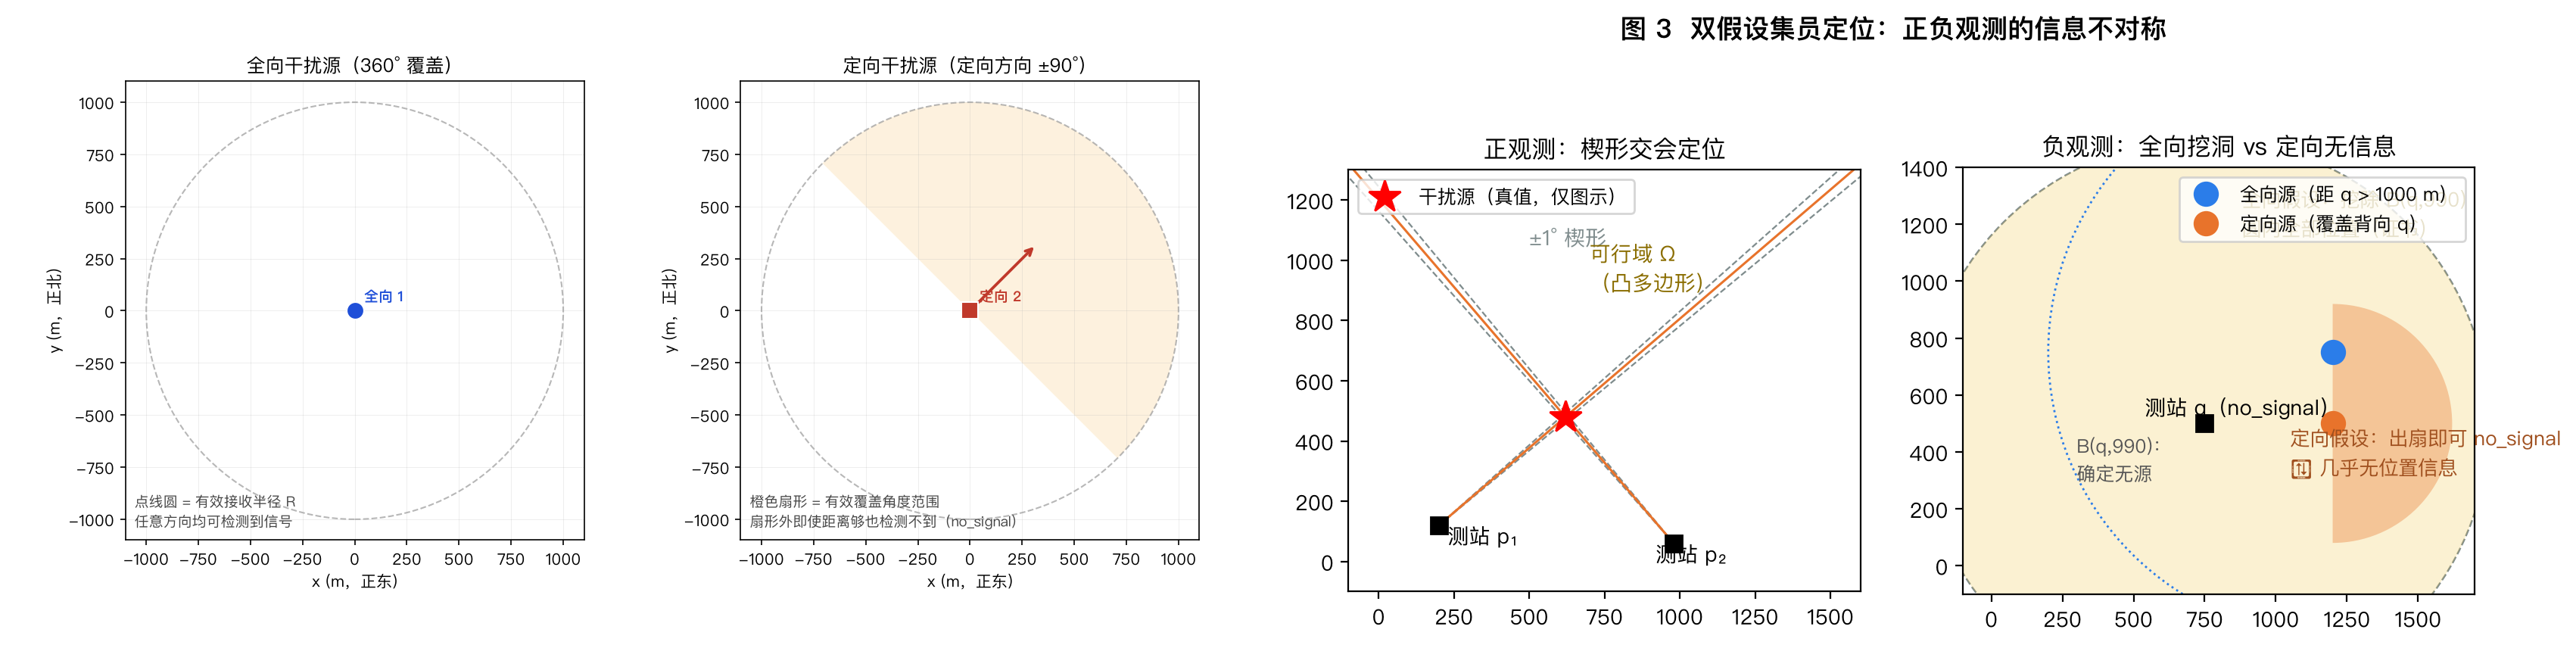
\includegraphics[width=0.96\textwidth]{p19_x136.png}
\caption{干扰源类型（左）与正负观测的信息不对称（右）}
\end{figure}

\subsubsection{创新机制一：N19 超凸包普查网络}
发现阶段需要“沉默即可认证为空”的证明。构造 N19 站网：原点 $(0,0)$ + 内圈半径 $1000\,\mathrm{m}$ 正六边形（6 站）+ 外环半径 $1825\,\mathrm{m}$ 正十二边形（旋转 $15^{\circ}$，12 站），共 19 站（图 10）。外环凸包半径达到 $1825\,\mathrm{m}$，严格包裹住 $1800\,\mathrm{m}$ 竞赛区域：紧贴圆边、朝向外侧的定向源，其可听半平面大部分落在圈外，只能从圆外听见。数值核验表明，最坏条件下对任意边缘朝外定向源的残余漏听率低于 $0.06\%$。

\begin{figure}[H]
\centering
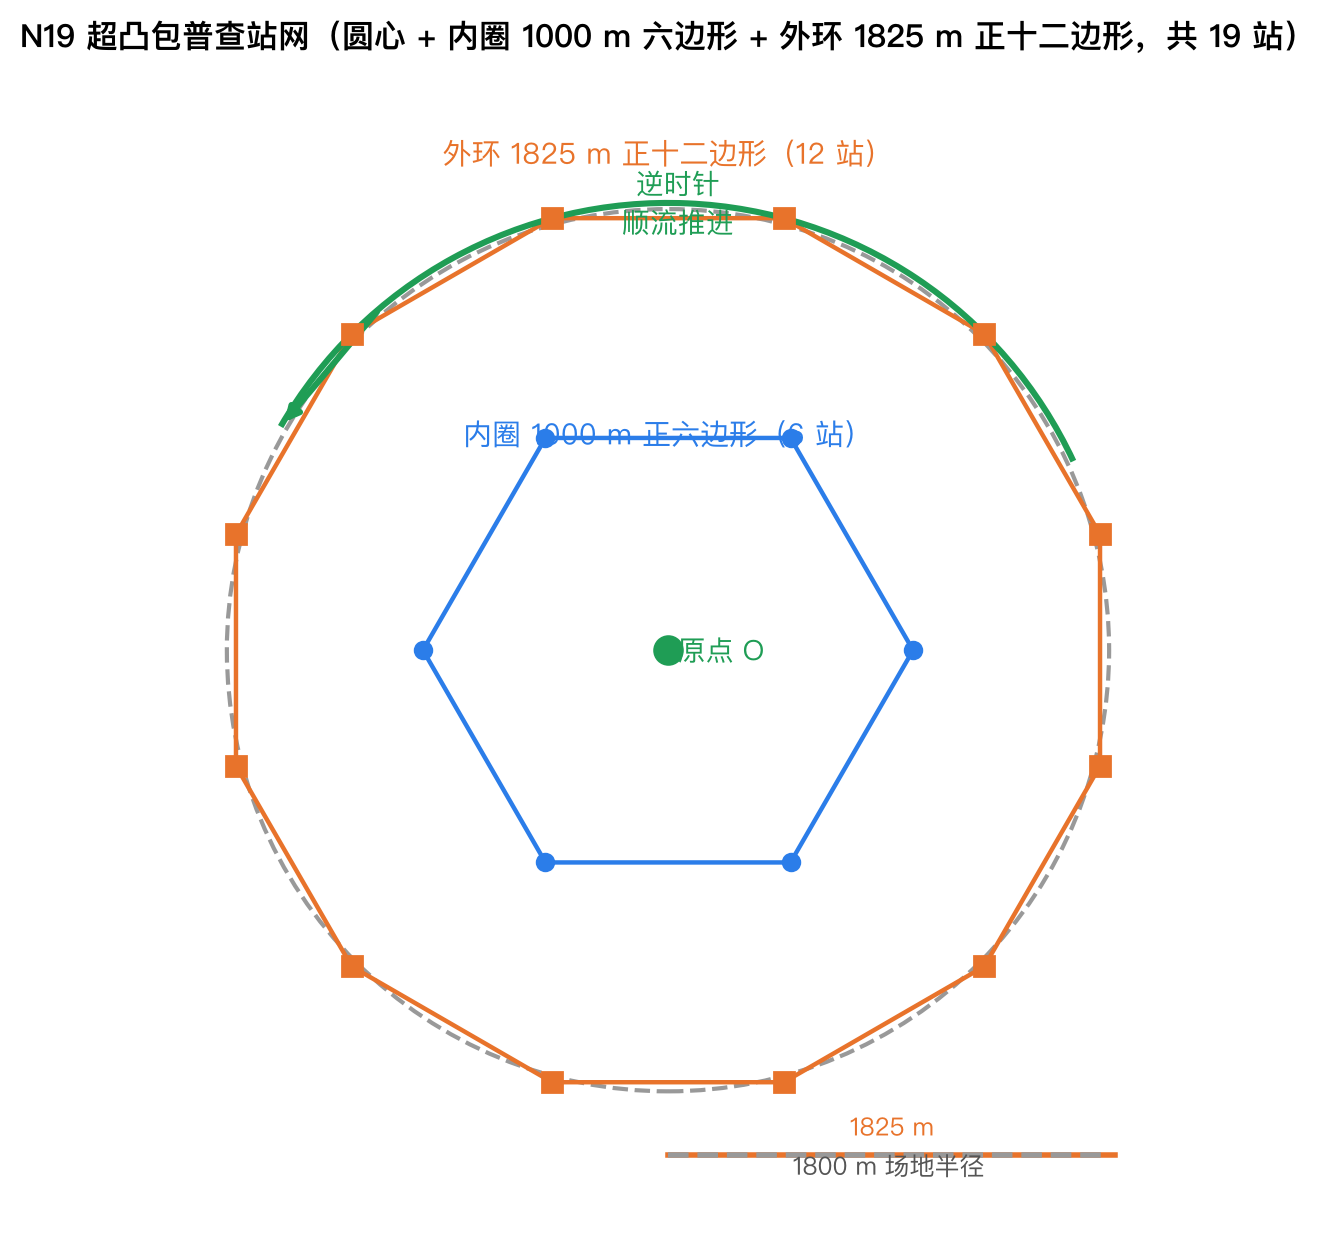
\includegraphics[width=0.58\textwidth]{p20_x141.png}
\caption{N19 超凸包普查站网（圆心 + 内圈 $1000\,\mathrm{m}$ 六边形 + 外环 $1825\,\mathrm{m}$ 正十二边形）}
\end{figure}

\subsubsection{创新机制二：逆时针单向顺流推进（CCW Flow）}
机器狗按逆时针由内向外巡检：内圈正六边形按逆时针普查结束后，顺势切入外环第一站（$15^{\circ}$ 偏角），保持单向角动量推进。相比反向顺时针切入（CW），避免了内外圈交界处的巨大折返过渡惩罚，实测单局净省 $1220\,\mathrm{s}$、少走 $4.6\,\mathrm{km}$（表 7）。

\subsubsection{创新机制三：$1300\,\mathrm{m}$ 扇区单向延迟收割}
传统贪心在外环巡检时，一旦锁定源就立即掉头折返跨越半个圆周去清，会引发灾难性的“跨半球拉锯跑”。本文规则：若目标在身后远端（逆时针夹角 $90^{\circ}{\sim}330^{\circ}$ 且距离 $>1300\,\mathrm{m}$），强制挂起延迟、禁止回头，保持外环单向推进，等环线自然巡检绕到该扇区邻近位置时顺路收割。实测平均少跑 $4.18\,\mathrm{km}$，局均净省 $641\,\mathrm{s}$（稀疏局暴省 $1313\,\mathrm{s}$）（表 6）。

\subsubsection{创新机制四：奔袭转场静默免听}
机器狗在赶路奔袭与补站交会过程中，仅测听正在追踪的活跃源，彻底屏蔽对未知频道的盲听；普查任务严格收敛于 19 个正规普查点，单局砍掉 8--10 次无效停测时间税。

整体算法流程如图 11 所示。

\begin{figure}[H]
\centering
\begin{tikzpicture}[
  font=\small\sffamily,
  >=Stealth,
  node distance=0.46cm and 0.20cm,
  box/.style={draw=black!60, rounded corners=2.2pt, align=center, inner sep=4.2pt, text width=8.6cm, fill=blue!4},
  task/.style={draw=black!60, rounded corners=2.2pt, align=center, inner sep=3.4pt, text width=2.22cm, minimum height=1.55cm, font=\footnotesize\sffamily},
  arr/.style={->, thick}
]
\node[box] (start) {开始：原点 $(0,0)$，频道 1};
\node[box, below=of start, fill=green!8] (n19) {N19 普查：内圈 $1000\,\mathrm{m}$ 六边形\\（6 站）逆时针巡回};
\node[box, below=of n19, fill=green!8] (outer) {外环 $1825\,\mathrm{m}$ 正十二边形（12 站）\\顺流切入，保持单向角动量};
\node[box, below=of outer] (replan) {每停任务池重规划\\（清除 / 补测 / 追踪）};
\node[task, fill=green!10, below=0.78cm of replan, xshift=-3.63cm] (t1) {$R_{\mathrm{MEC}}\le 20\,\mathrm{m}$\\清除任务};
\node[task, fill=blue!6, right=0.16cm of t1] (t2) {补测选点\\可听份额选点};
\node[task, fill=orange!8, right=0.16cm of t2] (t3) {扇区延迟收割\\身后远端挂起};
\node[task, fill=purple!6, right=0.16cm of t3] (t4) {奔袭静默免听\\只测活跃源};
\coordinate (fan) at ($(replan.south)+(0,-0.22)$);
\node[box, below=0.85cm of t2] (belief) {定向源状态：位置$\times$朝向网格\\{\ttfamily no\_signal} 按朝向衰减（不挖盘）};
\node[box, below=of belief, fill=green!8] (stop) {三模停机：听全 16 只 / 掩码空证书 /\\残余质量 $\le$ 阈值 $\to$ 结束};
\foreach \a/\b in {start/n19,n19/outer,outer/replan} \draw[arr] (\a) -- (\b);
\draw[thick] (replan.south) -- (fan);
\foreach \t in {t1,t2,t3,t4} \draw[arr] (fan) -| (\t.north);
\draw[arr] ($(t2.south)!0.5!(t3.south)$) -- (belief.north);
\draw[arr] (belief) -- (stop);
\draw[arr, red!70!black, thick] (belief.west) -- ++(-1.15,0) |- node[pos=0.25, left, font=\scriptsize\sffamily, text=red!70!black, align=right] {每停一次\\重规划} (replan.west);
\end{tikzpicture}
\caption{问题四算法整体流程（N19 + 逆时针顺流 + 扇区延迟收割 + 奔袭静默免听）}
\end{figure}

\subsubsection{三模自主停机（无上帝视角）}
终止规则完全基于信念、不读取剩余源数真值，三模停机：条件 A 累计听全 16 只干扰源（题面上限）；条件 B 所有未听频道的朝向掩码位全空（空证书）；条件 C 未听频道的后验残余质量均值 $\le 1\%$（$\varepsilon$-收敛停机）。

\subsubsection{求解结果}
（1）官方正式三次测试。在官方模拟器上三次正式测试均清除全部干扰源，结果见表 4。

\begin{table}[H]
\centering
\caption{问题四官方正式三次测试}
\small
\begin{tabular}{@{}ccccc@{}}
\toprule
\textbf{序号} & \textbf{清除数} & \textbf{总时间/s} & \textbf{平均清除时间/(s/源)} & \textbf{运行时间/s} \\
\midrule
1 & 12 & 6902.50 & 575.21 & 27.255 \\
2 & 11 & 6370.99 & 579.18 & 12.416 \\
3 & 15 & 8663.87 & 577.59 & 22.349 \\
\bottomrule
\end{tabular}
\end{table}

三次测试的单源耗时分别为 $575.21/579.18/577.59\,\mathrm{s}$（样本量 $n=3$），波动幅度 $0.69\%$；其中第 3 次抽到 15 源的重度极值大局，依然 $15/15$ 全部肃清。压力演练中 16 源顶格极值局达成 16 听 16 清、单源耗时进一步压低至 $470.09\,\mathrm{s}/$源，提前触发证书停机。

（2）1 万局大规模蒙特卡洛仿真。在未知源数量（10--16）、未知空间坐标、未知波束朝向（全向/定向各 $50\%$）下运行 10000 局高保真仿真，结果见表 5。

\begin{table}[H]
\centering
\caption{问题四 10000 局蒙特卡洛仿真评测结果}
\small
\begin{tabularx}{\textwidth}{@{}L{3.6cm}L{4.3cm}Y@{}}
\toprule
\textbf{统计指标} & \textbf{数值} & \textbf{说明} \\
\midrule
仿真规模 & 10000 局 & 10--16 源随机场景 \\
满清局数 / 满清率 & 9980 局 / $99.80\%$ & Wilson 95\% CI $[99.69\%,\,99.87\%]$ \\
干扰源总清除率 & $99.98\%$（$130319/130339$ 只） & 混合源宏观清除比例 \\
全向源专项清除率 & $100.00\%$ & 64957 只全向源无一漏检 \\
定向源专项清除率 & $99.97\%$（$65362/65382$ 只） & $180^{\circ}$ 隐蔽定向源捕获率 \\
满清局平均完成时间 & $6642.66\,\mathrm{s}/$局 & 中位 $6566.84\,\mathrm{s}$，P95 $7761.36\,\mathrm{s}$ \\
平均单源清除用时 & $521.15\,\mathrm{s}/$源 & 逐局平均口径，95\% CI $[519.41,\,522.88]$ \\
平均行进路程 & $23835\,\mathrm{m}/$局 & 约 $23.84\,\mathrm{km}$ \\
平均测向切频次数 & $303.17$ 次/局 & 采样总频次 \\
程序异常局数 & 0 & 全部 10000 局正常运行 \\
\bottomrule
\end{tabularx}
\end{table}

按每局源数 10--16 分组，各组满清率依次为 $99.85\%$、$99.79\%$、$99.93\%$、$99.93\%$、$99.72\%$、$99.65\%$、$99.73\%$，平均停止时间 $6443.9{\sim}6898.5\,\mathrm{s}$，随源数单调上升，不存在源数偏置。

（3）残留源机理剖析（核心亮点）。10000 局中 20 局未满清，且每局均仅剩 1 只定向源，全部走齐 19 个普查点后由 $\varepsilon$-收敛规则正常停机，全部全向源无一漏检。这说明算法在常规及绝大多数复杂场景下均能实现满清，仅在极少数“贴近场地边界且主瓣背向场内”的定向源几何奇点处存在极小漏检（发生率 $0.20\%$），从逆向印证了 N19 外环站网已逼近边界几何覆盖的理论极值。

（4）与问题三策略直接移植的对比（消融分析）。若将问题三算法直接移植至问题四（p3port 基线），由于全向负信息误挖洞与 7 点网对定向源存在 $25.3\%$ 覆盖盲区，清除率断崖式暴跌至 $24.1\%$（纯定向下仅 $5.3\%$）；本文的位置$\times$朝向集员滤波 + N19 完备普查网 + 扇区单向延迟收割将清除率提升至 $99.98\%$，彻底解决了定向源隐蔽性带来的挑战。

（5）典型运行轨迹。图 13 给出 12 只混合源（7 只定向、5 只全向，与正式测试 1 规模对齐）满清案例的完整轨迹：紫色扇区为定向源真实 $180^{\circ}$ 辐射范围，机器狗沿内圈 6 点建立粗测向集后，按逆时针单向顺流展开外环 12 点巡航，从侧翼“包抄”定向源主瓣并一次性延迟收割（清除点 $C_1\sim C_{12}$）；右图显示累计路程 $21.75\,\mathrm{km}$、单源均时 $528.3\,\mathrm{s}$，最终由动态朝向网格残余质量收敛停机。

\begin{figure}[H]
\centering
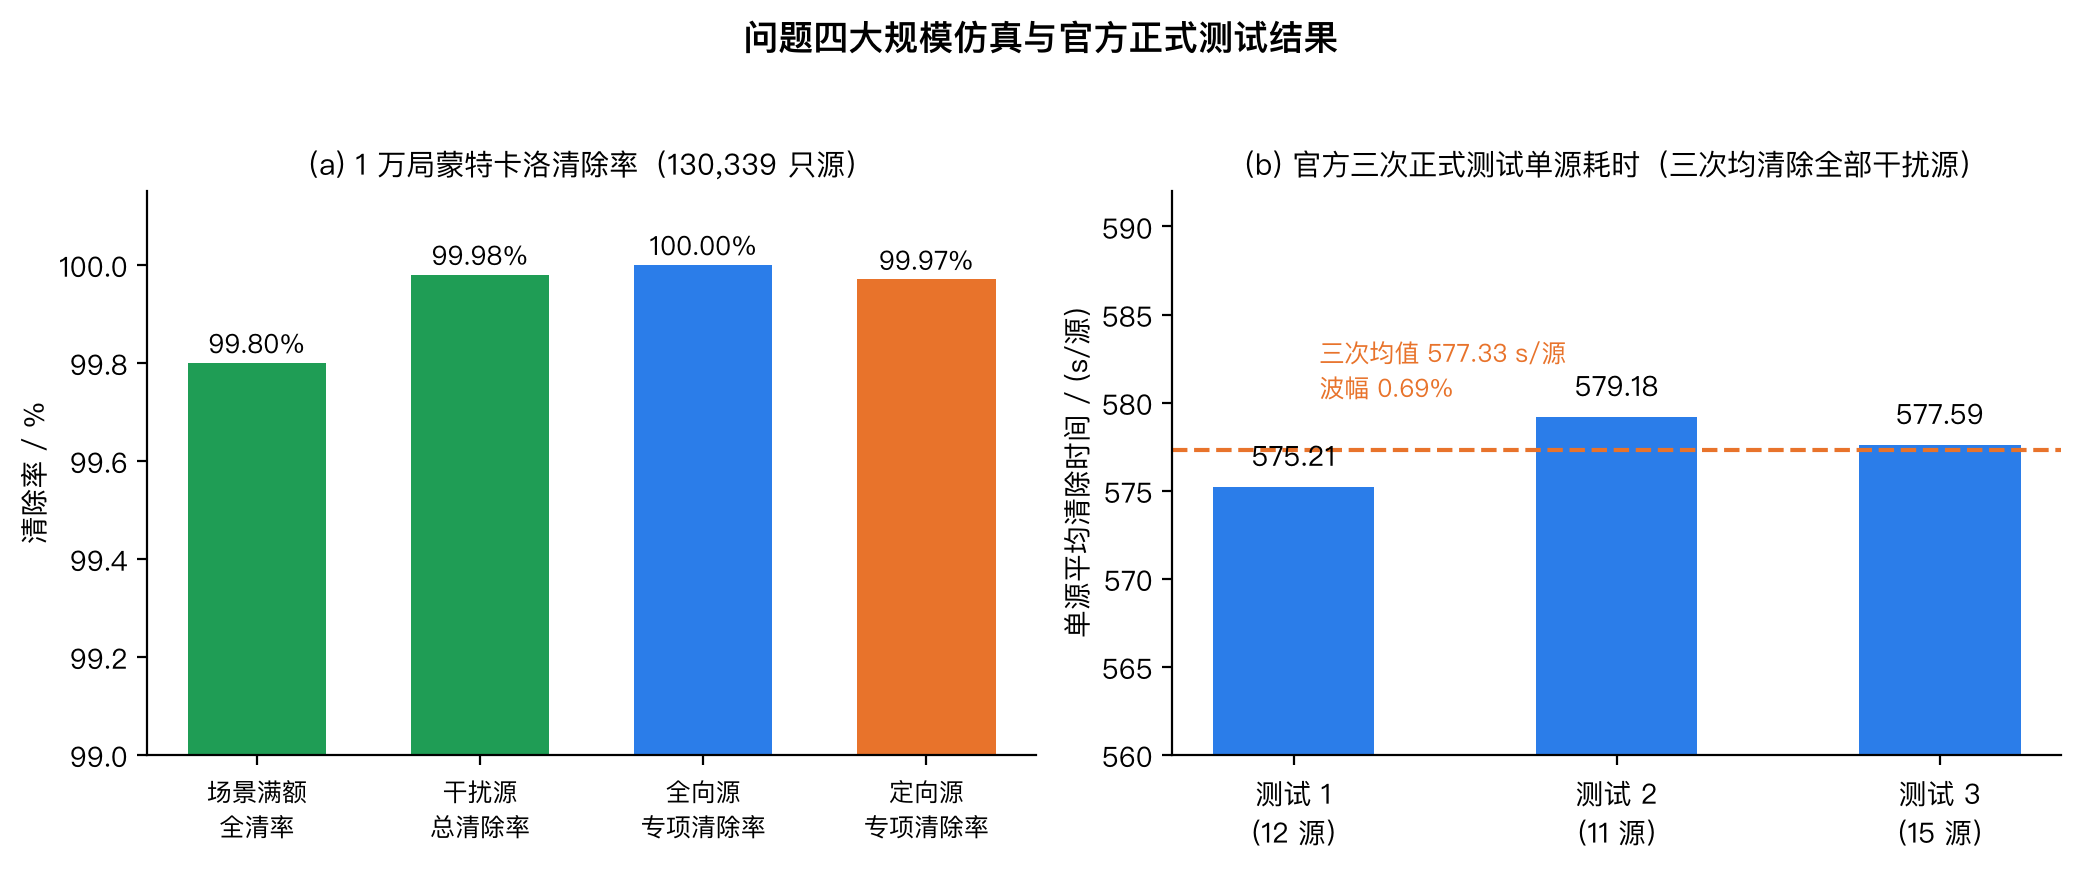
\includegraphics[width=0.96\textwidth]{p24_x160.png}
\caption{问题四 1 万局清除率与官方三次正式测试单源耗时}
\end{figure}

\begin{figure}[H]
\centering
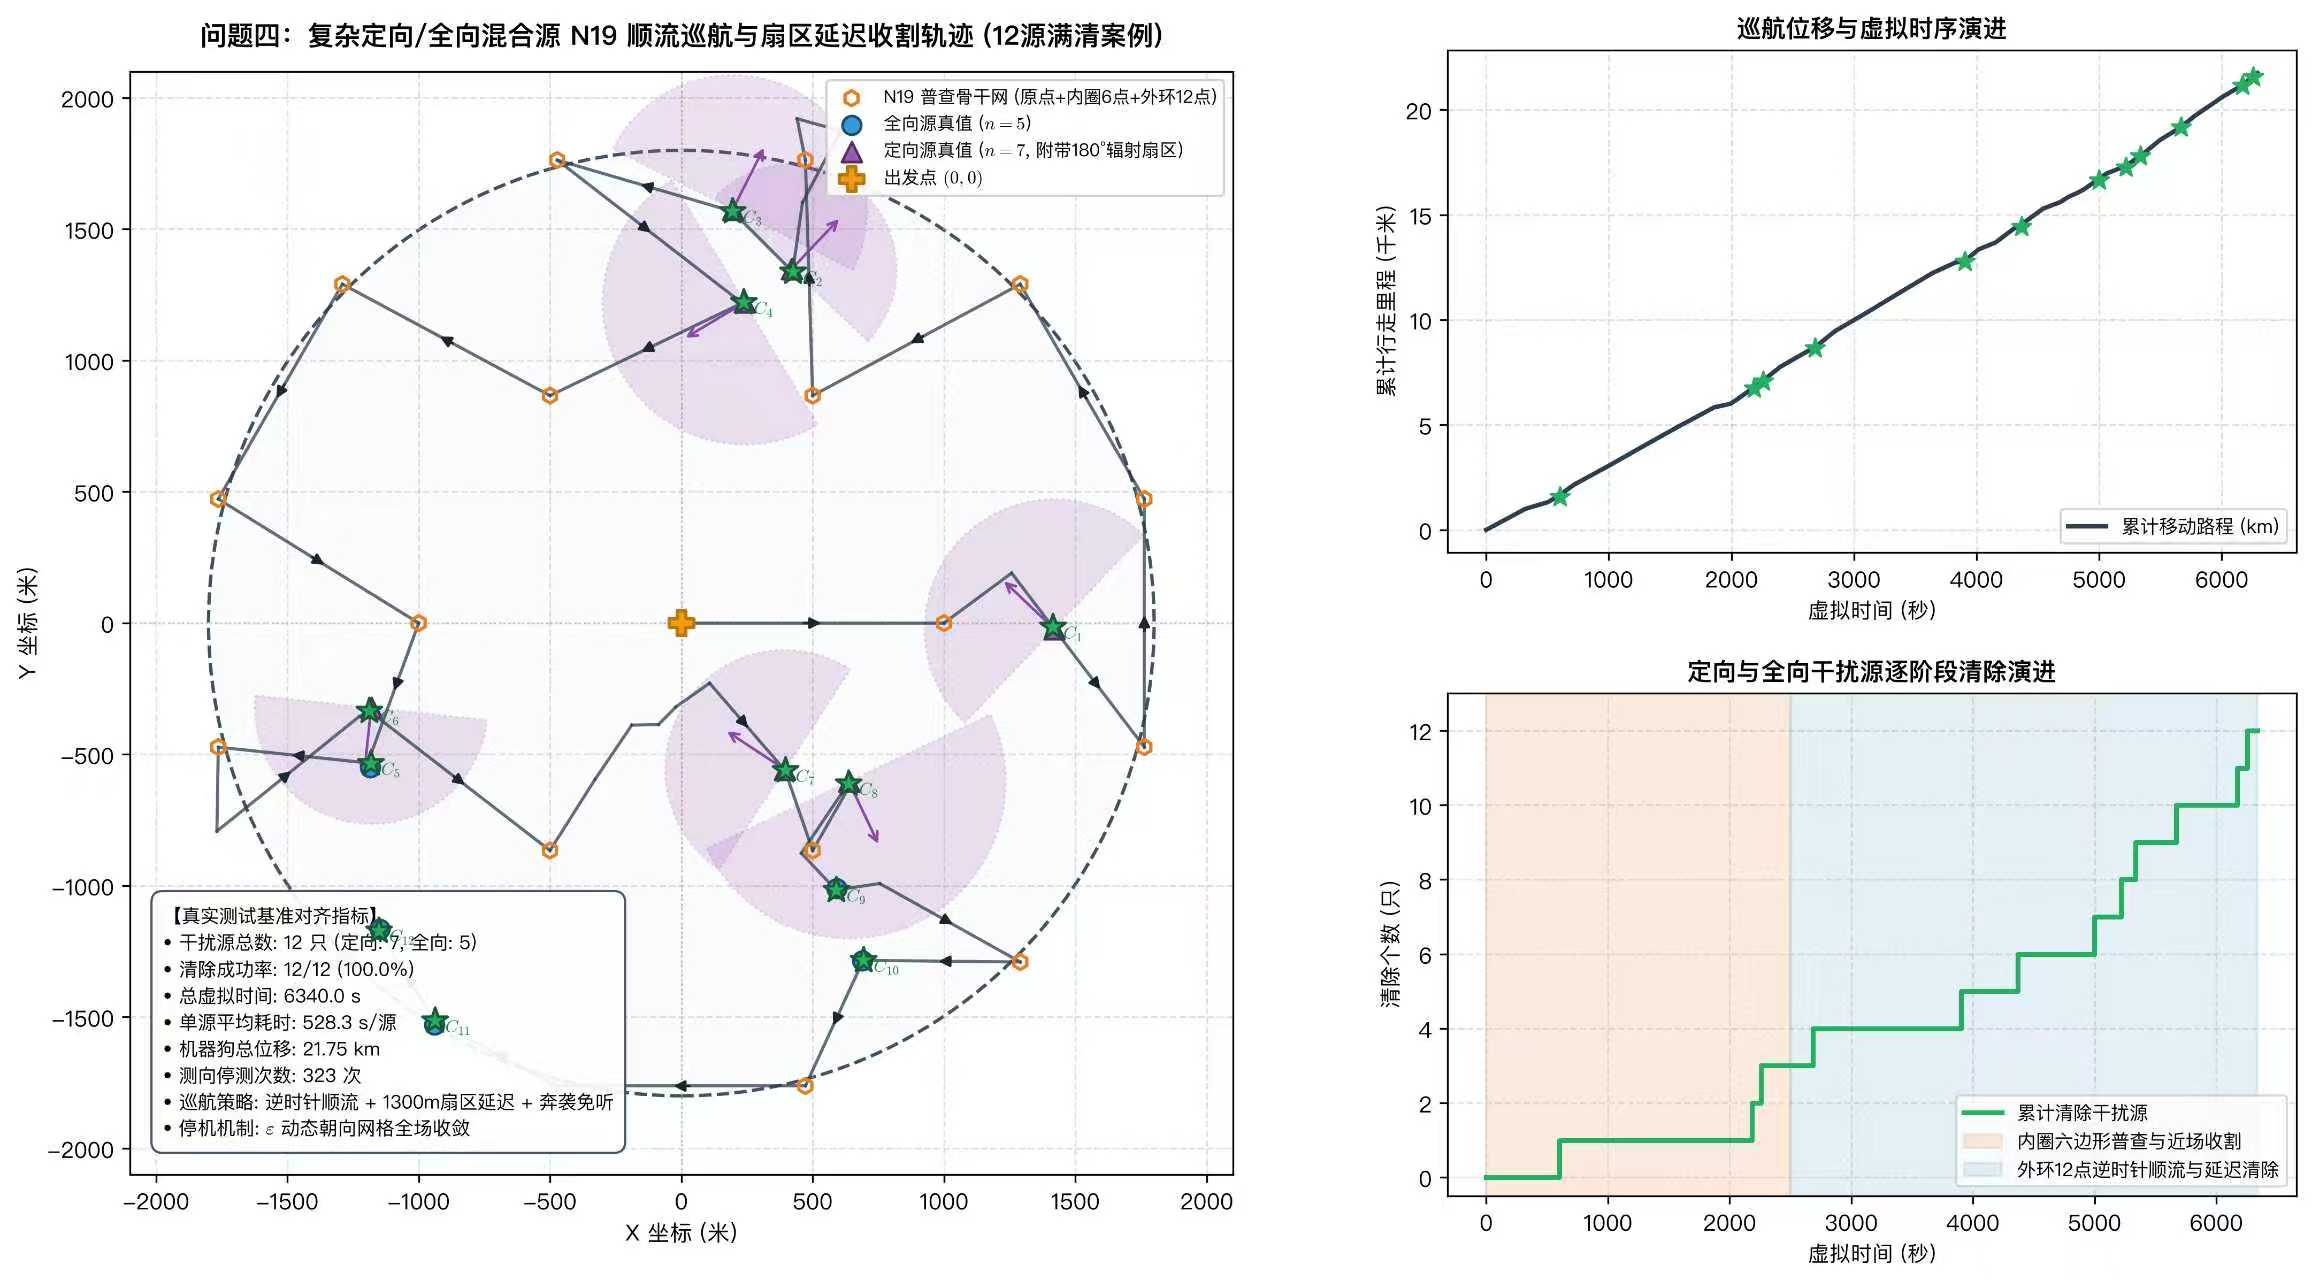
\includegraphics[width=0.92\textwidth]{p24_x161.jpeg}
\caption{问题四复杂定向/全向混合源 N19 顺流巡航与扇区延迟收割轨迹图}
\end{figure}

\section{模型检验与结果分析}
（1）问题一：已知形状解析验证。对等边三角形、正方形、长方形、直角三角形、正五边形、正六边形、正 36 边形用解析理论值验证，直径与最小包围圆的最大绝对误差约 $1.8\times 10^{-15}$；对 2000 组随机凸多边形，旋转卡壳与暴力枚举、Welzl 与暴力最小包围圆全部一致；对 10000 次随机真实源仿真，真实源 $100\%$ 落在计算出的定位区域内（5 次因区域无界被正确单列）。

（2）问题二：交叉验证与灵敏度。两套独立实现（不同几何引擎与采样方案）在共同候选点上重评，三构型最坏直径绝对差 $0.0017/0.0005/0.0052\,\mathrm{m}$，互证到毫米级；最坏情形一致出现在楔形远弧端点 $\times$ 误差极值处；容差 $\alpha\in[1.1,1.5]$ 时候选区域形状稳定，最优点向内回退约 $3\,\mathrm{m}$ 后 $J$ 仅增 $0.3\%$。

（3）问题三：覆盖网覆盖性与鲁棒性。7 点覆盖网最坏点距 $989\,\mathrm{m}<1000\,\mathrm{m}$，在最坏接收半径下保证每源至少被听见一次；10000 局中 5 个未清局均只剩 1 只源、都撞 160 步上限，属“听见之后锁不住”的定位边角情况而非覆盖网漏听；清完率 $95\%$ 置信区间 $[99.91\%,99.99\%]$；官方三次测试均正常停机、清除失败 0 次。

（4）问题四：消融实验与稳健性检验。三组严格同种子、同世界的配对消融实验验证了三大机制的真实收益：

\begin{table}[H]
\centering
\caption{扇区单向延迟收割消融实验（官方模拟器 6 对 6 局）}
\small
\begin{tabularx}{\textwidth}{@{}Ycccc@{}}
\toprule
\textbf{策略版本} & \textbf{满额全清率} & \textbf{平均总用时/s} & \textbf{平均路程/km} & \textbf{10 源局用时/s} \\
\midrule
原版贪心巡检（无扇区延迟） & $100\%$ & 7014.2 & 26.787 & 7236.0 \\
扇区延迟收割（本文） & $100\%$ & 6373.1 & 22.605 & 5923.0 \\
优化收益 & 维持 $100\%$ & 净省 $641.1\,\mathrm{s}$（$-9.1\%$） & 少走 $4.18\,\mathrm{km}$（$-15.6\%$） & 暴省 $1313\,\mathrm{s}$（$-18.1\%$） \\
\bottomrule
\end{tabularx}
\end{table}

\begin{table}[H]
\centering
\caption{外环巡检旋向消融实验（严格同种子配对）}
\small
\begin{tabularx}{\textwidth}{@{}L{2.0cm}cL{2.5cm}L{2.3cm}L{2.3cm}Y@{}}
\toprule
\textbf{场景种子} & \textbf{源数} & \textbf{逆时针顺流（本文）/s} & \textbf{顺时针反向/s} & \textbf{用时净收益} & \textbf{路程净收益} \\
\midrule
Seed 2027 & 10 & 6170.3 & 7390.9 & 净省 $1220.5\,\mathrm{s}$ & 少走 $4.62\,\mathrm{km}$ \\
Seed 2028 & 12 & 6340.0 & 6340.0 & 持平 & 持平 \\
Seed 2029 & 15 & 6100.9 & 6194.6 & 净省 $93.7\,\mathrm{s}$ & 少走 $573\,\mathrm{m}$ \\
Seed 2030 & 12 & 6819.1 & 6819.1 & 持平 & 持平 \\
\bottomrule
\end{tabularx}
\end{table}

逆时针巡检在所有局目中全面占优或持平，原因在于内圈正六边形普查按逆时针进行、结束后顺势切入外环第一站（$15^{\circ}$）保持角动量顺流。

\begin{table}[H]
\centering
\caption{延迟距离门限敏感性（$1300\,\mathrm{m}$ vs $1150\,\mathrm{m}$）}
\small
\begin{tabularx}{\textwidth}{@{}Yccccc@{}}
\toprule
\textbf{门限设置} & \textbf{Seed 2027/s} & \textbf{Seed 2028/s} & \textbf{Seed 2029/s} & \textbf{Seed 2030/s} & \textbf{平均路程/m} \\
\midrule
收紧（$1150\,\mathrm{m}$） & 6298.3 & 6340.0 & 6100.9 & 6819.1 & 22113.1 \\
基准（$1300\,\mathrm{m}$，本文） & 6170.3 & 6340.0 & 6100.9 & 6819.1 & 21924.2 \\
\bottomrule
\end{tabularx}
\end{table}

$1300\,\mathrm{m}$ 门限位于“防远端折返”与“就近顺路切入”的黄金分割点，收紧至 $1150\,\mathrm{m}$ 会迫使近场源滞后补清、多走 $755\,\mathrm{m}$。此外，官方三次正式测试的单源耗时波动幅度仅 $0.69\%$，在未知源数、未知朝向、$\pm 1^{\circ}$ 测向误差的黑盒世界中高度收敛于 $577\,\mathrm{s}/$源，验证了算法的强鲁棒性与抗随机性。

\section{模型评价与改进}
\subsection{模型优点}
\begin{enumerate}
\item 几何意义清晰、判据严格：角形区域到半平面的转化精确等价（引理 1），覆盖判定由定理 4 给出充要条件，有界性由衰退锥判据严格给出（定理 1），不引入人为截断；直径 $O(m)$、最小包围圆期望 $O(m)$、半平面交 $O(k\log k)$，可被在线策略高频调用。
\item 状态完备、数值口径诚实：显式处理空/有界/无界三态；问题二的 $J$ 如实标注为有限网格上确界估计，本地仿真与官方测试口径严格分离。
\item 在线决策闭环完整：每频道独立可行域的集员估计避免交叉误删，覆盖与追击混排、每停一次重规划显著缩短总时间（问题三较静态对照省 $38\%$）。
\item 可证明的完备性与机制创新：问题四的 N19 超凸包站网把“沉默”变成可证明的“空”（漏听率 $<0.06\%$），是 $99.98\%$ 清除率的根基；逆时针顺流、扇区延迟收割、奔袭静默免听三大机制在消融实验中分别带来 $641\,\mathrm{s}$、$1220\,\mathrm{s}$ 的真实收益。
\item 可对接性与可推广性：决策只依赖接口返回值、不读模拟器真值，可直接对接官方接口；框架可推广至多智能体协同搜索、未知辐射源监测等“信息获取与行动执行耦合”场景。
\end{enumerate}

\subsection{模型局限与改进方向}
\begin{enumerate}
\item 问题一：区域构造为 $O(n^{3})$，检测点很多时效率低于 $O(n\log n)$ 经典半平面交算法；未建模误差相关性（同一地点重复测量误差不独立）；未考虑定向干扰源的覆盖角约束。
\item 问题二：$J$ 为有限网格上的最坏值估计，连续上确界与连续全局最优尚未严格认证；按有界最坏情形处理偏保守；仅演示三个典型构型。
\item 问题三：覆盖网按最坏接收半径 $1000\,\mathrm{m}$ 设计偏保守；任务较多时开路哈密顿路退化为 2-opt 启发式；仍有 5 局（$0.05\%$）“听见之后锁不住”。
\item 问题四：依赖“无遮挡、无随机漏检”的官方规则前提；延迟收割门限（$1300\,\mathrm{m}$）与朝向网格分辨率（64 角）为经验参数；1 万局中仍有 $0.20\%$ 的“贴边背向”几何奇点漏检（均为单只定向源）。
\end{enumerate}
改进方向：以区间算术对问题二做连续全局最优认证；为问题三剩余未清局设计沿可行域长轴定向扫掠的兜底搜索；对问题四的“贴边背向”奇点增设边界外侧定向补听环，并自适应调节延迟收割门限。

\section{结论}
本文针对无线电干扰源快速自动定位与清除问题，按“交会定位---检测点选取---在线搜索清除”的递进层次建立了四个问题的数学模型，主要结论如下：
\begin{enumerate}
\item 问题一：建立“角形区域---半平面---凸多边形”的交会定位模型，用旋转卡壳求直径、Welzl 求最小包围圆，证明“存在直径为 $D$ 的圆覆盖定位区域当且仅当 $\Rmec=D/2$”，7 种已知形状验证误差约 $10^{-15}$ 量级，10000 次仿真真实源包含率 $100\%$。
\item 问题二：推导保证接收域 $\Crecv$ 与最坏交会直径目标 $J$，三构型最优直径 $111.0/41.0/8.2\,\mathrm{m}$，最优第二检测点“贴外沿、偏角约 $40^{\circ}$”，以 1.25 倍近最优水平集给出候选区域，两套实现互证到毫米级。
\item 问题三：提出“每频道可行域 + 覆盖混排 + 每停重规划”在线策略，官方三次测试清除 16、13、12 个源、平均定位清除时间 $220.28/258.65/250.17\,\mathrm{s}$，本地万局清完率 $99.95\%$、较静态对照省时 $38\%$。
\item 问题四：建立位置$\times$朝向联合网格的集员状态表示与 N19 超凸包普查站网，配合逆时针顺流、扇区延迟收割、奔袭静默免听三大机制；官方三次测试单源耗时 $575.21/579.18/577.59\,\mathrm{s}$（波幅 $0.69\%$），本地 1 万局满清率 $99.80\%$、总清除率 $99.98\%$、全向源 $100.00\%$，平均单源耗时 $521.15\,\mathrm{s}/$源。
\end{enumerate}
四个问题层层递进：问题一为全部定位计算奠基，问题二提供粗定位依据，问题三、四将几何定位嵌入在线决策闭环，在官方模拟器与本地仿真上稳定实现高清除率与短总时间。本文模型几何意义清晰、判据严格、决策只依赖接口返回值，可为“信息获取与行动执行耦合”的在线决策问题提供通用框架。

\section*{AI 工具使用声明}
\addcontentsline{toc}{section}{AI 工具使用声明}
本参赛队在竞赛过程中使用了 AI 工具，主要用于语言润色、代码调试与图表绘制辅助，详细使用情况见支撑材料《AI 工具使用详情》。所有 AI 生成内容均经队员逐项人工审查与核实。

\clearpage
\section*{参考文献}
\addcontentsline{toc}{section}{参考文献}
\begin{enumerate}[leftmargin=1.8em,itemsep=0.28em,label={[\arabic*]}]
\item Welzl E. Smallest enclosing disks (balls and ellipsoids)[C]//New Results and New Trends in Computer Science, LNCS 555. Berlin: Springer, 1991: 359-370.
\item Toussaint G T. Solving geometric problems with the rotating calipers[C]//Proceedings of IEEE MELECON'83. Athens, 1983: A10.02/1-4.
\item Preparata F P, Muller D E. Finding the intersection of $n$ half-spaces in time $O(n\log n)$[J]. Theoretical Computer Science, 1979, 8(1): 45-55.
\item Megiddo N. Linear-time algorithms for linear programming in $R^{3}$ and related problems[J]. SIAM Journal on Computing, 1984, 13(4): 759-776.
\item Li P, Liu Y, Yan T, et al. An underwater source localization method using bearing measurements[J]. Sensors, 2024, 24(5): 1627.
\item Land A H, Doig A G. An Automatic Method of Solving Discrete Programming Problems[J]. Econometrica, 1960, 28(3): 497-520.
\item Torrieri D J. Statistical theory of passive location systems[J]. IEEE Transactions on Aerospace and Electronic Systems, 1984, AES-20(2): 183-198.
\item Milanese M, Vicino A. Optimal estimation theory for dynamic systems with set membership uncertainty: an overview[J]. Automatica, 1991, 27(6): 997-1009.
\item Bezdek K. \"{U}ber einige Kreis\"{u}berdeckungen[J]. Beitr\"{a}ge zur Algebra und Geometrie, 1983, 14: 7-13.
\item Held M, Karp R M. A dynamic programming approach to sequencing problems[J]. Journal of the Society for Industrial and Applied Mathematics, 1962, 10(1): 196-210.
\item Arkin E M, Hassin R. Approximation algorithms for the geometric covering salesman problem[J]. Discrete Applied Mathematics, 1994, 55(3): 197-218.
\item Schweppe F C. Recursive state estimation: unknown but bounded errors and system inputs[J]. IEEE Transactions on Automatic Control, 1968, 13(1): 22-28.
\item Nardone S C, Lindgren A G, Gong K F. Fundamental properties and performance of conventional bearings-only target motion analysis[J]. IEEE Transactions on Automatic Control, 1984, 29(9): 775-787.
\end{enumerate}

\clearpage
\section*{附录}
\addcontentsline{toc}{section}{附录}
\subsection*{附录 A\quad 支撑材料文件列表}
\begin{itemize}
\item 问题一：\texttt{问题一/问题一代码final\_修正版.py}（半平面交 + 旋转卡壳 + Welzl + 覆盖判定 + 仿真检验）、\texttt{问题一\_表格与图像.py}、\texttt{problem1\_localize.py}、\texttt{figs/}（示向度、交会定位、角形区域及验证图）。
\item 问题二：\texttt{问题二/code/problem2\_model.py}、\texttt{problem2\_paper.py}、\texttt{problem1\_localize.py}、\texttt{test\_problem2.py}、\texttt{final\_refine.py}、\texttt{results/problem2\_summary.json}、\texttt{figs/}（三张候选区域图）。
\item 问题三：\texttt{问题三/code/}（\texttt{problem3\_belief\_struct.py}、\texttt{problem3\_belief.py}、\texttt{problem3\_route\_solver.py}、\texttt{run\_official\_e15.py}、\texttt{problem3\_official\_robot.py} 等上场源程序）、\texttt{正式日志/}（三份 \texttt{formal-p3-*.jlog} 及表 1）、\texttt{本地结果/}（fullopt 1 万局 \texttt{summary.json}/\texttt{trials.csv}，E15 本地 1000 局摘要）。
\item 问题四：\texttt{问题四/code/}（\texttt{problem4\_belief\_n19.py}、\texttt{run\_official\_n19.py} 及依赖源程序）、\texttt{正式测试成绩.txt}（三次官方成绩；未附 \texttt{formal-p4-*.jlog}）、\texttt{本地结果/}（N19 本地 1000 局 \texttt{summary.json}/\texttt{trials.csv}）。
\item AI 工具使用详情：\texttt{AI工具使用详情.pdf}。
\end{itemize}

\subsection*{附录 B\quad 源程序代码}
完整、可运行的源程序代码见支撑材料，本附录不全文粘贴。

\end{document}
